\documentclass[ABmsc, twoside, ABpages, % ABproject,
ABfinal, 
 ABfig, ABgraph,  ABprog, ABtab, ABalg, ABgls, ABroom, ABbib, ABindex,% ABnatbib,  %ABdraft  
]{ABThesis}
% !TeX root=main.tex
%برای گرفتن خروجی در مقطع دکتری لطفا پارامتر ABmsc را از خط اول حذف کنید.
%برای اجرای نمایه به صورت خودکار خط فرمان زیر را بدون % در مسیر 
%Options/Configure Texmaker/Quick Build
%جایگزین نمایید ضمنا خصوصیت ABindex در خط ۳ بایست فعال کنید.
% دقت داشته باشید که با این روش هر بار نمایه بروز می‌شود اما سرعت اجرا را کاهش می‌دهد. لذا در صورت عدم تمایل به استفاده خصوصیت ABindex را بردارید.
%xelatex --shell-escape -interaction=nonstopmode -synctex=-1 %.tex

\begin{document}
\renewcommand{\arraystretch}{1}

%\marginpar{ زندگی تنها به این درد می خورد که انسان به دو کار مشغول شود، اول ریاضیات بخواند، دوم ریاضیات درس بدهد.   \\  ژاکوب ژاکویی}\\


\ifABpages
\renewcommand{\baselinestretch}{1}\normalsize
% دانشگاه خود را وارد کنید
\university{نام دانشگاه‌تان}
% دانشکده، آموزشکده و یا پژوهشکده  خود را وارد کنید
\faculty{دانشکده محل تحصیل‌تان}
% گروه آموزشی خود را وارد کنید
\department{نام گروه آموزشی‌ که در آن تحصیل می‌کنید}
% رشته آموزشی خود را وارد کنید
\subject{نام رشته‌تان}
% گرایش خود را وارد کنید
\field{گرایش‌تان}
% عنوان پایان‌نامه را وارد کنید
\title{راهنمایی بر پایان‌نامه/رساله نویسی با تِک\;\TeX}

% نام استاد(ان) راهنما را وارد کنید
\firstsupervisor{دکتر}
%\secondsupervisor{دکتر}
% نام استاد(دان) مشاور را وارد کنید. چنانچه استاد مشاور ندارید، دستور پایین را غیرفعال کنید.
\firstadvisor{دکتر}
%\secondadvisor{دکتر}
\TSupervisor{جناب آقای دکتر}
\TAdvisor{سرکار خانم دکتر}
\TOArbiter{جناب آقای دکتر}
\TTArbiter{سرکار خانم دکتر}


% نام پژوهشگر را وارد کنید
\name{گروه دانشجویی ابوالوفا}
% نام خانوادگی پژوهشگر را وارد کنید
\surname{بوزجانی}
% تاریخ پایان‌نامه را وارد کنید
\thesisdate{فروردین ماه 1400}
\okdate{1399/6/1}
\defencedate{1399/7/1}
% کلمات کلیدی پایان‌نامه را وارد کنید
\keywords{رساله، پایان‌نامه، تک، راهنما}
% چکیده پایان‌نامه را وارد کنید
\abstract{
حداکثر در حجمی معادل با 250 تا 300 کلمه تهيه شده و شامل بيان مختصر مسئله مورد بررسی، روش تحقيق و مراحل بکار گرفته شده برای کسب و جمع آوری اطلاعات، نحوه تجزيه و تحليل و نتيجه کلی می باشد. خواننده با مطالعه چکيده بايد تشخيص دهد که رساله موجود دربرگيرنده مطالب مورد علاقه وی می باشد يا خير؟ تاريخچه و سابقه موضوع در اين قسمت ذکر نشده، بلکه در مقدمه رساله توضيح داده می شود. چکيده در يک صفحه مجزا قبل از فهرست مطالب قرار می گيرد . در بالای آن به فاصله دو سطر از حاشيه بالای صفحه در ميانه سطر عنوان پايان نامه نوشته می شود. در انتهای چکيده ميتواند کلمات کليدی مورد استفاده در پايان نامه به تعداد 5-4 واژه اضافه شود. \\
دوستان شما در این رساله سعی دارند تا شما را با یک قالب پایان‌نامه/ رساله آشنا کنند. شما با توجه به همین بسته موجود (ABThesis) و راهنمایی‌های ارائه شده در این نمونه رساله خواهید توانست با اندکی دقت ضمن یاد گرفتن اصول فنی نوشتن تحت \TeX با نگارش فنی نیز آشنا شوید، لازم به ذکر است که قالب حاضر به طور اختصاصی استانداردهای دانشگاه فردوسی را پشتیبانی می‌کند. \\
لازم به ذکر است که ما تعداد کلمات در چکیده به طور رسمی دارای محدودیت است از این‌رو ما نیز با توجه به آن فضای مربوط به چکیده‌مان را تنظیم کردیم.
}

\baselineskip=.6cm
\latinuniversity{Ferdowsi University of Mashhad}
\latinfaculty{Faculty of Mathematical Sciences}
\latinsubject{Pure Mathematics}
\latinfield{Mathematical Analysis}
\latintitle{The probabilistic powerdomain for stably compact spaces}
\firstlatinsupervisor{First Supervisor}
%\secondlatinsupervisor{Second Supervisor}
\firstlatinadvisor{First Advisor}
%\secondlatinadvisor{Second Advisor}
\latinname{English name}
\latinsurname{English family}
\latinthesisdate{2020}
\latinokdate{2020}
\latindefencedate{2020}
\latinkeywords{Probabilistic powerdomain; Stably compact space; Valuation}
\latinabstract{
This thesis reviews the one-to-one correspondence between stably compact spaces (a topological
concept covering most classes of semantic domains) and compact ordered Hausdorff spaces. The
correspondence is extended to certain classes of real-valued functions on these spaces. This is the
basis for transferring methods and results from functional analysis to the non-Hausdorff setting.
}



\pagestyle{empty}
\besm{besm}
\ftitle
%صورتجلسه بایست به امضای دانشجو و اساتید برسد و سپس اسکن آن به صورت پی‌دی‌اف در کنار فایل‌های دیگر با نام minutes ذخیره شود.

\includepdf{minutes}
\specifications
%اصالت‌نامه بایست به امضای دانشجو و اساتید راهنما برسد و سپس اسکن آن به صورت پی‌دی‌اف در کنار فایل‌های دیگر با نام originality ذخیره شود. فایل خام آن را می‌توانید از پوشه other بردارید.
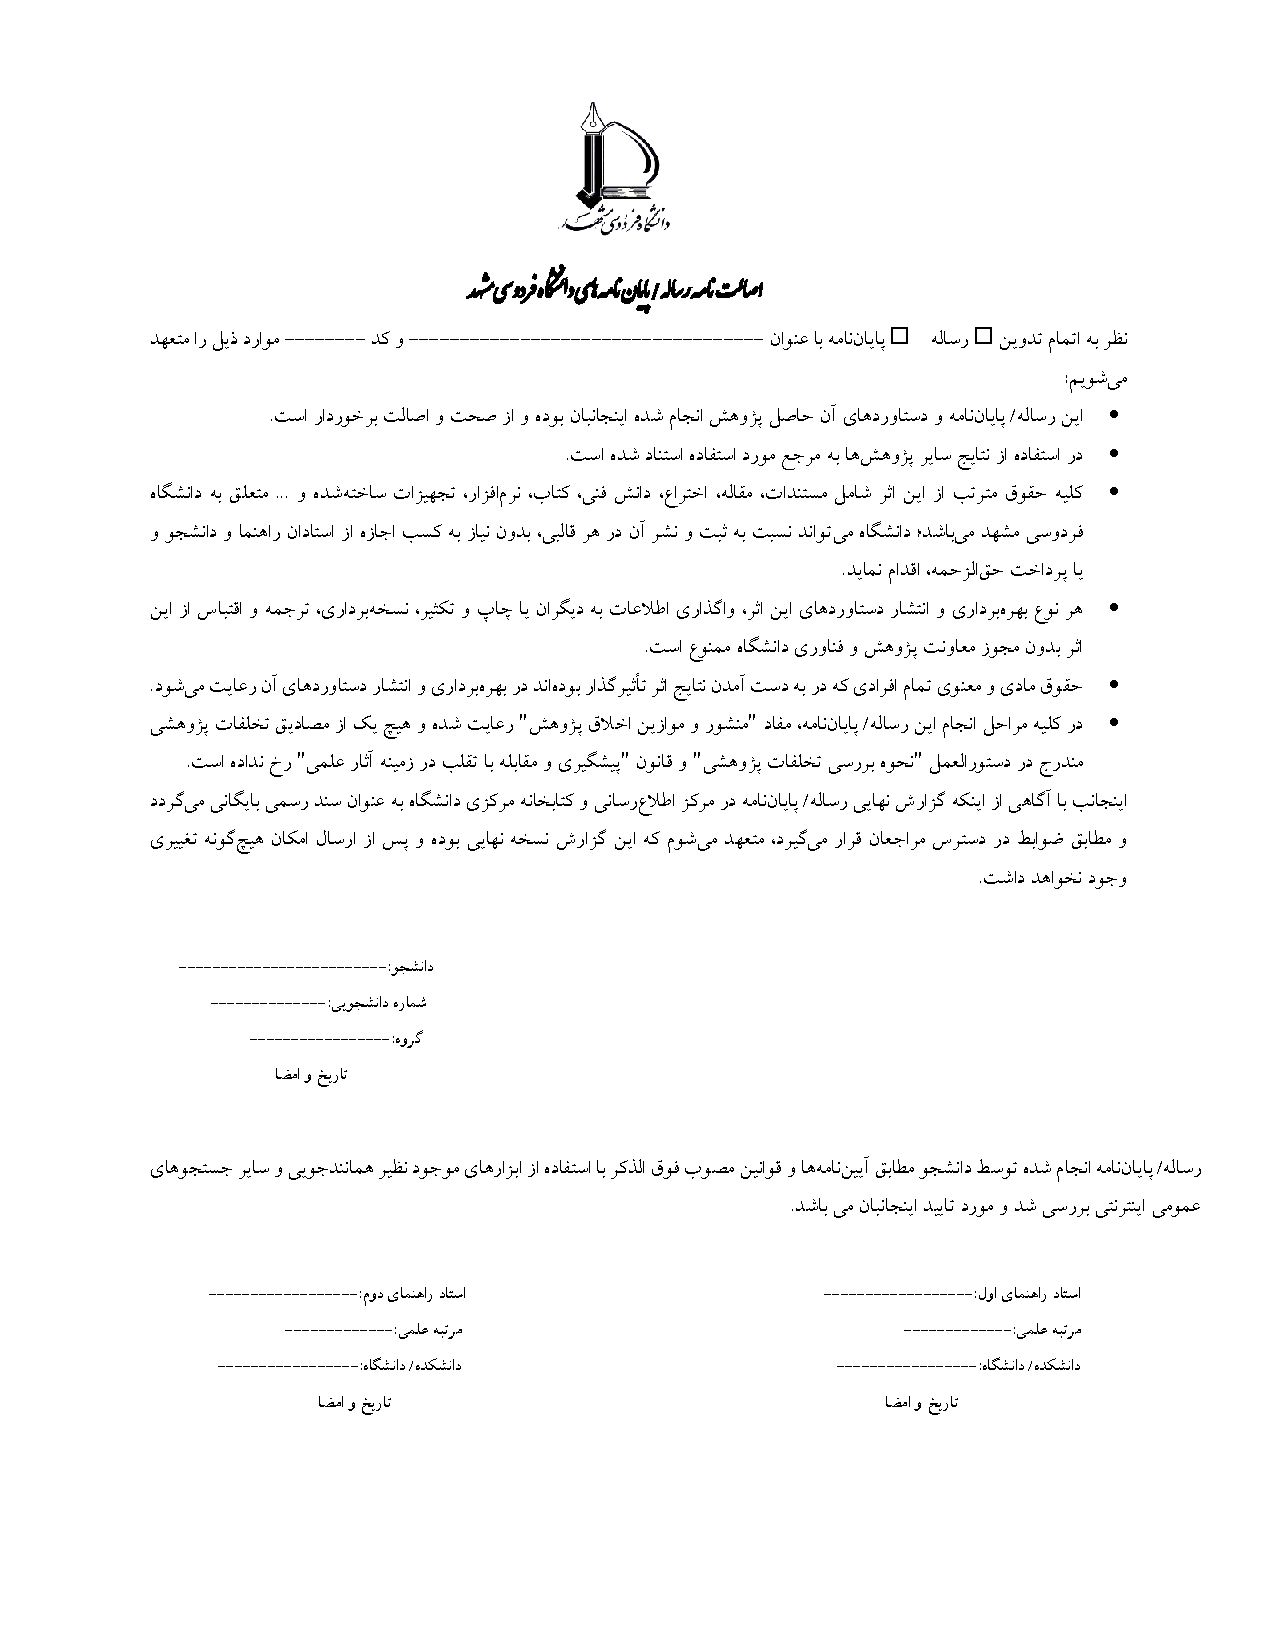
\includepdf{originality}
\presentation{1}{تقدیم به }{...}{که ...}
\praise{1}{هوالعلیم،}{به نام حق که ...\\}{می‌کوش به هر ورق که خوانی \hspace*{\fill} تا معنی آن تمام دانی}
\thanks{1}{سپاس‌گزاری}{سپاس خداوند بلندمرتبه\\}{نام}‮‮



%در صورتی که مایل به استفاده از فهرست نماد هستید عبارت‌های مربوط به محیط comment را در خط بعد و خط آخر این فایل حذف کنید. لازم به ذکر است که از دو نوع فهرست نماد هر کدام را که مایل هستید می‌توانید استفاده کنید و دیگری را بایست حذف نمایید. 
\begin{comment}
\newpage
\begin{center}
\tos{فهرست نمادها و علائم ریاضی}{%
\srow{جمع}{$\sum$}
\srow{ضرب}{$\prod$}
\srow{تقسیم}{$/$}
}{2} 
\end{center}

\begin{center}
\tos{فهرست نمادها و علائم ریاضی}{%
\srow{جمع}{$\sum$}{s1}
\srow{ضرب}{$\prod$}{s1}
\srow{تقسیم}{$/$}{s1}
}{3}
\end{center}
برای این‌که فهرست نمادها را به کارتان اضافه کنید کافی‌ست بعد از انتخاب یکی از دو جدول فوق بقیه سطرها را به انتخاب خودتان تکمیل کنید. شاید اساسی‌ترین نکته دقت در به کار بردن فهرست سه ستونه است که برای استفاده از آن شما باید در جایی که نماد برای بار اول به کار برده می‌شود از دستور label استفاده کنید و برای تکمیل جدول فقط پارامتری که  هنگام استفاده از label استفاده کرده‌اید را بنویسید.
$\sum\label{s1}$
\pagebreak
\end{comment}‮
\else\relax\fi

\clearpage
\pagenumbering{alph}
%\pagestyle{plain}
%\baselineskip=.75cm
\renewcommand{\baselinestretch}{1.9}\normalsize
\phantomsection\addcontentsline{toc}{chapter}{فهرست مطالب}
\tableofcontents



\ifABpages
\listoffigures
\listoftables
%\listofdiagrams % if uncomment this command(\listofdiagrams) must uncomment "ABroom" in end of line 4
\ifABalg
\listofalgorithms % if uncomment this command(\listofalgorithms) must uncomment "ABroom" in end of line 4
\else\relax\fi
\else\relax\fi









\certificate{۳۱۳۰۱}{همکار محترم با ذکر کد خود ایرادات مربوط به کار مشتری را در ابتدای سند درج بفرمایید.}

\abovedisplayshortskip=0pt
\belowdisplayshortskip=0pt
\abovedisplayskip=4pt
\belowdisplayskip=4pt


\pagestyle{fancy}
\begin{preface}[مقدمه]
یادآوری می‌کنیم که پیش گفتار معمولا شامل اهمیت موضوع، پیش‌زمینه، طرح مسئله تحقیق و انجام ضرورت آن، مرور مفصل پیشینه موضوع و مقایسه پایان‌نامه با پژوهش‌های مشابه از نظر محتوا و روش تحقیق، اهداف عمده تحقیق و محدودیت‌های خارج یا تحت کنترل آن است.\footnote{پیش‌گفتار ما را بخوانید و ارزیابی‌مان کنید. آیا موفق بوده‌ایم؟}

به سبب رشد نرم‌افزار نوپای زی‌پرشین\LTRfootnote{\XePersian} در ایران و تنوع و پیچیدگی کار نیاز به یک راهنمای کوتاه و جامع و به روز را احساس کردیم، چرا که تا آن‌جا که یافتیم به روزترین راهنما ترجمه‌ی دکتر امیدعلی به نام مروری نه چندان کوتاه بر لاتک بود که مجموعه‌ای جامع است اما با توجه به نیازهایی که خودمان در طول چندین سال تجربه با آن مواجه بودیم بر آن شدیم که موجز و مفید از نصب تا تکمیل کار را به صورت عملی در این پایان‌نامه بیان کنیم. ضمن اینکه در همین راستا به معرفی قالب طراحی شده برای دانشکده ریاضی دانشگاه فردوسی مشهد بپردازیم، که نسخه‌ای مطابق با استانداردهای دانشکده بوده و متناسب با نیازها بر پایه قالب تغییر یافته آقای وحید دامن‌افشان از روی قالب Thesisی ست که توسط آقای دکتر وفا خلیقی طراحی شده است.



اما آن‌چه که در شروع کار بایست به آن توجه داشته باشید، این است که راهنمای حاضر به هیچ وجه به عنوان راهنمایی بر لاتک یا زی‌پرشین مطرح نیست، که نه دانش نویسنده در این حد است و نه مجالی آن‌چنان که بتوان محتوایی بدون ایراد و درخور توجه نگاشت. هدف تنها مرقوم داشتن تجربه‌ای ست که به نظر می‌رسد می‌تواند در صرفه‌جویی زمان دانشجویانی که فقط قصد نگارش پایان‌نامه‌شان به زبان پارسی و با استفاده از نرم‌افزار زی‌پرشین را دارند، موثر باشد.


دیگر آنکه توجه کنید این راهنما را بایست بتوانید تولید نمایید چون عملا بهره‌ی مفیدی که می‌توان از آن برد در گرو این است که قادر باشید خروجی‌ای مشابه فایل راهنما با اجرای فایل main.tex داشته باشید. البته به شرط آن‌که مطابق آن‌چه در فصل\ref{c1} گفته می‌شود مراحل نصب را انجام داده باشید. در این صورت کافی‌ست یک دور مطالعه کنید و بعد از آن با گرفتن یک کپی از فایل‌های موجود(به عنوان پشتیبان تا در صورت لزوم دوباره بتوانید به آن‌ها رجوع کنید) محتوای مورد نظرتان را در اسناد مربوطه جایگزین کنید.


لطفا توجه کنید که این مجموعه فقط برای دانشکده ریاضی دانشگاه فردوسی آماده شده پس اگر آن را برای ارائه به جای دیگری استفاده کنید لازم است خودتان تغییرات لازم را انجام دهید، چون هر دانشگاهی یک سری تنظیمات خاص دارد و اصلا دلیل این‌که این بسته به صورت واحد ایجاد نشده همین تنوع و تفاوت استانداردها در دانشگاه‌های مختلف است.

خوب حال که قرار بر این شد که فایل‌های منبع موجود با این راهنما را نیز مطالعه کنید، انتظار داریم که شما فایل‌های tex مربوطه را نیز در هر قسمت ملاحظه کنید. پس لازم می‌دانیم یادآوری کنیم که توضیحات اضافی مربوط به هر قسمت از سند به صورت توضیح در هر یک از فایل‌های تک آورده شده که بد نیست در طول کار آن‌ها را به دقت مورد مطالعه قرار دهید تا کمتر دچار مشکل شوید.

ما
\begin{description}
\item[در فصل اول]
 این رساله به بیان روش‌های نصب و آپدیت تک‌لایو ۲۰۱۱ در سیستم عامل ویندوز خواهیم پرداخت البته امیدواریم در آینده نزدیک مجال آن را داشته باشیم تا مراحل نصب در لینوکس و دیگر سیستم عامل‌های مطرح را داشته باشیم.
\item[در فصل دوم]
به بیان یک سری مطالب برگرفته از راهنمای math mode خواهیم پرداخت که راهنمای تنظیماتی است که تحت بسته‌های AMS\footnote{متعلق به انجمن ریاضی آمریکا} قابل دسترسی‌اند که به خصوص در ریاضی‌نویسی با آن سروکار خواهید داشت.
\item[در فصل سوم]
به معرفی چند بسته کاربردی برای رشته‌های آمار، ریاضیِ محض و ریاضیِ کاربردی خواهیم پرداخت.
\item[در فصل چهارم]
به نصب و تنظیمات زیندی برای تولید واژه‌نامه، نمایه و نیز قالب‌های فارسی برای تولید مراجع خواهیم پرداخت.
\end{description}
\end{preface}
\pagenumbering{arabic}
\def\bs{$\backslash$}
\chapter{راهنماهای نصب}
\section{نصب تک‌لایو}
به دو طریق می‌توانید تک‌لایو ۲۰۱۱ را نصب کنید.
\begin{enumerate}
\item
با استفاده از منبع برنامه که ممکن است با دی‌وی‌دی یا فلش به دست شما رسیده باشد، اما دانشجویان دانشگاه فردوسی می‌توانند نسخه نصبی را از اول مهر ماه ۹۰ آن را از مسیر \lr{ftp://}، در داخل شبکه دانشگاه نیز دانلود کنند.
\item
با استفاده از اینترنت
\end{enumerate}
\subsection{نصب از روی منبع}
در این روش شما باید سه مرحله زیر را انجام دهید.
\begin{enumerate}[a.]
\item
مطابق شکل زیر روی \lr{0\_texlive\_2011.exe} کلیک کنید و در پنجره‌ای که باز می‌شود ok را کلیک کنید تا فایل فشرده استخراج شود.(توجه داشته باشید که برای انتقال فقط از همان نسخه فشرده استفاده کنید، چون در غیر این‌صورت باید زمان زیادی صرف کنید)\\
در ادامه برای شروع فرآیند نصب بایست به داخل پوشه \lr{texlive} بروید و سپس فایل \lr{install-tl.bat} را اجرا کنید، در این زمان بایست طی حداکثر چند دقیقه یک پنجره سیاه‌رنگ باز شود و پس از آن صفحه خوش‌آمدگویی تک‌لایو ۲۰۱۱ که به شکل زیر است.

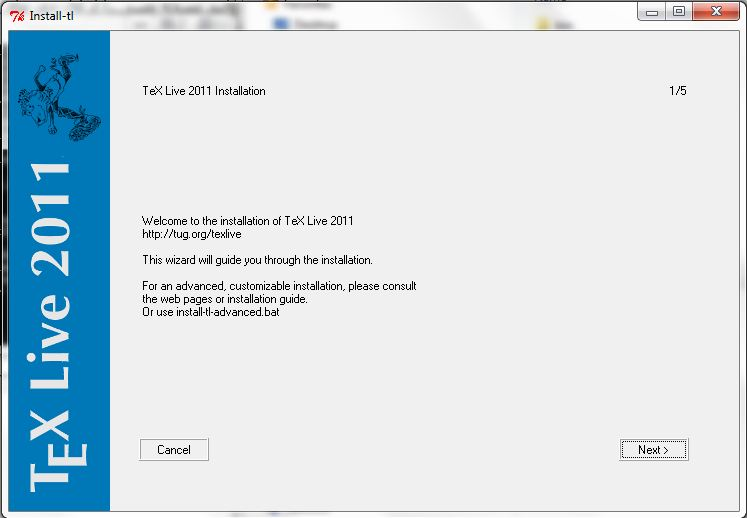
\includegraphics[scale=.5]{fig/welcome}

در ادامه راه شما فقط باید بدون تغییر هیچ چیز فقط به مراحل بعدی نصب بروید(عملا در سه پنجره اولی که باز می‌شوند فقط کافی‌ست \lr{next} و در پنجره چهارم هم \lr{install} را باید کلیک کنید.\\
بعد از انجام این مراحل دو صفحه یکی سیاه رنگ و دیگری آبی‌-خاکستری دارید که بسته‌های در حال نصب را نمایش می‌دهند. ۳۰ تا ۴۵ دقیقه که بگذرد دیگه باید نصب بسته‌ها تموم بشه و زیر صفحه دکمه \lr{finish} ظاهر بشه، روی اون کلیک کنید. در این‌جا مرحله اول تمام می‌شود و تک‌لایو به طور کامل نصب شده است.(نصب تک‌لایو در حقیقت اصلی‌ترین مرحله است و روح کار است در مراحل بعدی شما فقط ورودی برای استفاده از آن خواهید ساخت)
\item
در این مرحله باید ادیتور \lr{Texmaker} را نصب کنید(با نصب ادیتور شما می‌توانید از تک‌لایو نصب شده استفاده کنید، به این صورت که فایل را در ادیتور باز کرده و با اجرای آن ادیتور با اتصال به تک‌لایو تبدیل فایل متنی کد را به فایل پی‌دی‌اف ممکن می‌سازد) برای انجام این کار کافی‌ست شما به پوشه \lr{1\_Texmaker} بروید و تنها فایل درون آن به نام 
\lr{Texmaker\_BiDi-0.6.10\_STATIC\_installer.exe} را اجرا کنید و بدون هیچ تغییری فقط موافقت‌تان با نصب برنامه را اعلام کنید و تا آخر ادامه دهید.(تا این‌جا ادیتور هم نصب شد)
\item
در مرحله آخر فقط باید فونت‌های لازم را از  پوشه \lr{2\_FarsiFonts} به پوشه \lr{C:\bs Windows\bs Fonts} کپی کنید.
\end{enumerate}
خسته نباشید، شما به پایان نصب رسیدید. حال کافی‌ست یک فایل آماده با توسعه‌ی \lr{tex} را باز کرده و با زدن فلش آبی کنار \lr{QuickBuild} فایل را اجرا کرده و بعد از اتمام اجرا با زدن فلش آبی کنار \lr{ViewPDF} خروجی را مشاهده کنید. اما این فایل نمونه را که یک نمونه رساله برای دانشگاه فردوسی مشهد است را ما در پوشه‌ای به نام \lr{FThesis} آماده کرده‌ایم که شما بایست فایل \lr{main.tex} را از داخل آن انتخاب و در ادیتور \lr{Texmaker} اجرا کنید.
\subsection{نصب مستقیم با اینترنت}
در این روش شما به صورت مستقیم وارد مراحل نصب می‌شوید، بدیهی است که چنانچه در طول فرآیند نصب اتصال شما به اینترنت قطع شود دوباره باید نصب را از سر بگیرید.\\
این روش به زودی تشریح می‌شود.
\subsection{نصب غیرمستقیم با اینترنت}
در این روش شما ابتدا فایل‌های نصب را از اینترنت تهیه کرده و بعد به نصب از روی آن خواهید پرداخت. در این روش لزومی ندارد که حتما در یک بار اتصال تمام دریافت فایل انجام شود.\\
این روش به زودی تشریح می‌شود.
\section{تغییراتی که بایست برای استفاده از بیمر به صورت فارسی داده شود}
بیمر بسته‌ای برای طراحی اسلاید است که با زی‌پرشین سازگار نیست و با بسته جدید لواپرشین که برای رفع نواقص زی‌پرشین(از جمله عدم پشتیبانی همین بسته کارامد بیمر) اقدام به تولید آن شده است، سازگار است.

برای نصب شما بایست  مرحله زیر را انجام دهید.
\begin{enumerate}
\item
نصب لواپرشین.\\
به دایرکتوری \lr{C:\bs texlive\bs 2011\bs texmf-dist\bs tex\bs lualatex} بروید چنانچه پوشه‌ای به نام \lr{luapersian} دیدید و نیز فایلی به نام \lr{luapersian.sty} را درون آن یافتید بدانید که این بسته نصب شده در غیر این صورت بایست خودتان پوشه \lr{luapersian} را از پوشه \lr{beamer} همراه با این راهنما برداشته و در مسیری که در بالا گفتیم قرار دهید(\lr{C:\bs texlive\bs 2011\bs texmf-dist\bs tex\bs lualatex}) تا این جا نصب لواپرشین به اتمام رسیده و برای تست آن بایست حتما یک‌بار سیستم را ریست کنید(البته راه ساده‌تری هم برای اهل فن هست).
\item
در این مرحله شما باید فایلی به نام \lr{beamerbasetheorems.sty} را که برای تولید محیط‌های شماره‌دار فارسی دست‌کاری شده و در پوشه \lr{beamer} همراه با این راهنماست را با فایلی که با همین نام و در مسیر \lr{C:\bs texlive\bs 2011\bs texmf-dist\bs tex\bs latex\bs beamer} قرار دارد تعویض کنید(گفتیم تعویص تا اگر خواستید از بیمر در متون انگلیسی استفاده کنید دوباره با همین تعویض امکانش مهیا باشد، چون در حقیقت فایل \lr{beamerbasetheorems.sty} پیش‌فرض برای محیط لاتین و فایل \lr{beamerbasetheorems.sty} دست‌کاری شده توسط ما برای محیط فارسی مناسب است.)
\item
تنها کاری که مانده این است که تک‌میکر را برای اجرای لواپرشین آماده کنید، به این منظور به سراغ \lr{TeXmaker} رفته و از منوی \lr{Options} یا معادل فارسی آن \lr{Configure Texmaker} یا معادل فارسی آن را برگزینید. در پنجره‌ای که باز می‌شود و در سمت چپ آن بر روی شکلک \lr{Commands} کلیک کنید و در خط اول مقابل \lr{LaTeX}، عبارت \hbox{\lr{lualatex -interaction=nonstopmode -synctex=-1\; \%.tex}} را به طور دقیق بنویسد حال برای اجرا فایل امتحانی به سراغ فایل \lr{main} در پوشه \lr{sample}، در پوشه \lr{beamer} همراه این راهنما بروید. آن را با \lr{TeXmaker} باز کنید و با تنظیم اجرا قرار دادن نوار اجرا بر روی \lr{LaTeX} فلش آبی کنار آن را برای اجرا و فلش آبی بعد از آن را برای دیدن خروجی کلیک کنید.
\begin{center}
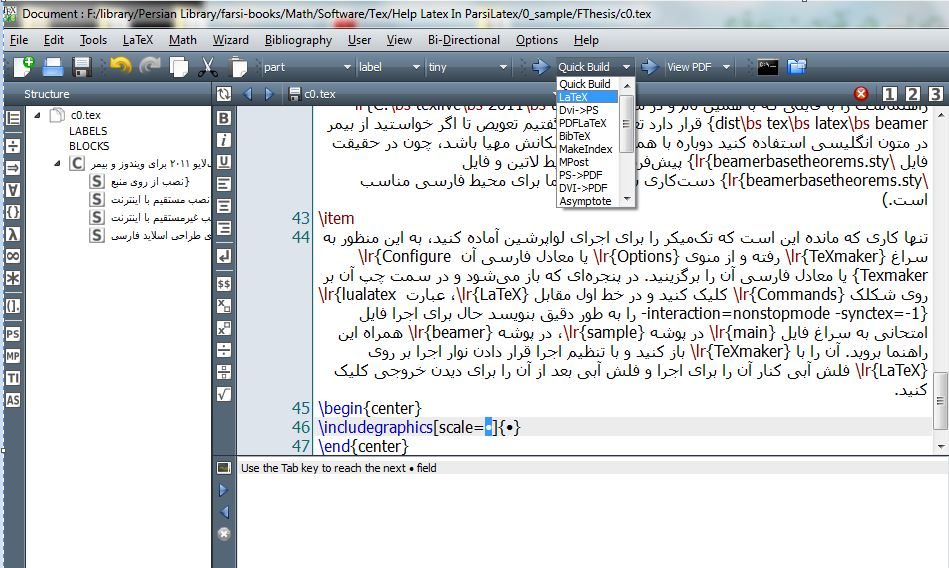
\includegraphics[scale=.3]{fig/beamer}
\end{center}
\end{enumerate}
\section{راه‌اندازی xindy برای تولید نمایه}
برای ایجاد نمایه شما لازم است ۴ فایل را برای اضافه کردن زبان فارسی اضافه کنید. این فایل‌ها در پوشه‌ای به نام \lr{persian} در پوشه \lr{TeX\;Pakage} قرار دارند، آن‌ها را در مسیر \lr{C:\bs texlive\bs 2011\bs texmf\bs xindy\bs modules\bs lang\bs} کپی کنید و بعد \lr{Command\;Prompt} را باز کنید و دستور \lr{texhash} را بزنید و مقداری تامل کنید تا عبارت \lr{done} را ببینید. حال اگر \lr{bidiTeXmaker} نسخه 3.1.0-3 را طبق دستورات بالا نصب کردید به سراغ منوی \lr{Tools} بروید و دستور \lr{Xindy Make Index} را برای تولید فایل مربوط به نمایه اجرا کنید و سپس فایل را اجرا کنید و خروجی را ببینید.%install
\chapter[ریاضی‌نویسی با نگاهی بر بسته AMS]{ریاضی‌نویسی با نگاهی بر بسته \inpdic{انجمن ریاضی آمریکا (AMS)}{American Meteorological Society}}
\section{بسته‌ها}
خوب \TeX یک زبان برنامه‌نویسی ست که برای حروف‌چینی اسناد آماده شده است. اما بسته به چه معناست: بسته‌ها یک سری ماکروهای از پیش نوشته شده هستند که خیلی از خصوصیات مورد استفاده در آن‌ها تعریف شده و بصورت
 مختصر به منظوراستفاده ی راحت تربرای افرادی که آشنایی با \TeX ندارند آماده‌سازی شده‌اند و در مخازن مربوط نگهداری شده و هر روزه همراه با راهنماهای مربوط در حال بروزرسانی‌اند.

اساسی‌ترین بسته برای ما پارسی‌زبانان بسته
\XePersian
است که پشتیبانی پارسی را در تک انجام می‌دهد و به همت دکتر وفا خلیقی تهیه شده است. لازم به ذکر است این بسته دیگر به روز نخواهد شد و آینده متعلق به لواپرشین است که به امید خدا پس از آماده‌سازی و تکمیل نهایی مبنای کار قرار خواهد گرفت که از جمله امکانات آن پشتیبانی از بسته قوی بیمر برای تهیه اسلاید است، لازم به‌ذکر است که نسخه آزمایشی آن هم‌اکنون در مسیر جاری نصب \TeX موجود بوده و قابل استفاده است. تاکنون متوجه شدیم که برخی بسته‌ها در \TeX نیز ممکن است با هم سازگار نباشند.

اما از دیگر بسته‌های پرکاربرد می‌توان بسته های تهیه شده توسط انجمن ریاضی آمریکا را نام برد که به طور معمول با ams شروع می‌شوند. در این فصل تلاش ما بر این است که با تکیه بر راهنمای آماده شده به نام mathmode که از راهنماهای موجود نصب شده همراه با \TeX می‌باشد، توضیحاتی را در جهت سهولت و افزایش کیفیت قسمت‌های ریاضی سندتان ارائه نماییم.

قبل از شروع لازم به یادآوری‌ ست که برای طرح مشکلات و کسب اطلاعات بیشتر در این خصوص می‌توانید به تالار گفتگوی پارسی لاتک در تارنمای  \lr{http://www.parsilatex.com/forum/SMF/index.php} مراجعه نمایید.

\section{محیط‌های ریاضی}
این یک نمونه است که موجز بودن در تهیه آن در اولویت قرار دارد پس به دقت همه چیز را در نظر بگیرید.

دوباره یادآوری می‌کنیم که ما اصلا قصد نداریم که تمام جزییات را برای‌ شماشرح دهیم، چون منابع موجود در این زمینه را کافی می‌دانیم و تلاش‌مان این است که فقط به شبیه‌سازی مواردی که ممکن است نیاز داشته باشید بپردازیم تا بتوانید بدون توجه به جزییات زیادی و تنها با کمی دقت و تامل خروجی مطلوب را داشته باشید.

ابتدا لازم است بدانید که ما به طور کلی محیط‌های متنوعی\footnote{منظور محیط‌هایی برای رسم ماتریس‌ها، آرایه‌ها، عبارات شماره‌دار و درون‌خطی و ...} برای نوشتن ریاضی در سندمان داریم.

\begin{definition}[دو محیط ریاضی اولیه]
دو محیط ریاضی رایج در \TeX داریم که قبل از هر چیز بایدبا آن آشنا شوید.
\begin{enumerate}
\item[$\$x\$ $]
فرمول‌های درون متنی\\
که بجای $x$ هر عبارت ریاضی می‌تواندقرار بگیرد.\\   
این فرمول‌ها  با یک جفت دلار مشخص می‌شوند. با زدن اولین دلار زبان به لاتین تغییر کرده و با بستن آن دوباره فارسی می‌شود. به عنوان مثال \verb|$\sum$|، که نمایش آن به صورت $\sum$ خواهد بود.

\item[$\backslash\rm{[} x \backslash\rm{]}$]
فرمول‌های نمایش(برون متنی)\\
جای $x$ چه می گذاریم؟
در این مورد با دو حالت مواجه هستیم:
\begin{enumerate}[ا.]
\item
بدون شماره\\
در این حالت از \verb|\] \sum \[| استفاده می‌شود. که خروجی آن به صورت زیر است.
\[\sum2\]
\item
با شماره\\
در این حالت از دستور \verb|equation| به صورت زیر استفاده می‌کنیم.

\begin{LTR}
\begin{verbatim}
\begin{equation}
\sum
\end{equation}
\end{verbatim}
\end{LTR}
که خروجی آن به صورت زیر است.
\begin{equation}
\sum
\end{equation}
\end{enumerate}
\end{enumerate}
\end{definition}


\begin{theorem}[عبارت‌های چند خطی تراز شده]
برای تراز کردن عبارت  های چند خطی از محیط \verb|\align| استفاده می‌شود.\\
مثلا برای داشتن خروجی
\begin{align}
4+5\times 2&=4+5+5\cr
&=4+10\cr
&=14.
\end{align}

باید به صورت زیر بنویسیم:
\begin{LTR}
\begin{verbatim}
\begin{align}
4+5\times 2&=4+5+5\cr
&=4+10\cr
&=14.
\end{align}
\end{verbatim}
\end{LTR}

\begin{description}
\iq
به نظر شما آیا این شماره‌گذاری منحصر به فرد است؟
\ia
اگر پاسخ‌ شمامثبت است لازم است حداقل برای تمرین هم که شده به فایل مراجعه کنید.
\begin{align}
4+5\times 2&=4+5+5\cr
&=4+10\\
&=14.\nonumber
\end{align}
آیا قانع شدید که هر کاری می‌شودانجام داد؟
\begin{align}
4+5\times 2&=4+5+5\label{eq4.2}\\
&=4+10\cr
&=14.\label{eq5.2}
\end{align}
\end{description}
\begin{description}
\iq
خوب حالا چه طور می‌شود برچسب برای این یکی ساخت؟
\ia
خوب به کدام قسمت آن می‌خواهید ارجاع بدهید؟ \eqref{eq4.2} یا \eqref{eq5.2}؟ 
\end{description}

برای عدم شماره گذاری کافی‌ست \verb|align|به \verb|align*| درآغازوپایان محیط تغییر دهیم. این روش برای عناوین و دیگر محیط‌ها نیز برقرار است.
\begin{description}
\iq
آیا فکر می‌کنید دیگر به تمام امکانات این محیط مسلط شده‌اید؟ حتما با این مسأله روبرو بوده اید که بخواهید با یک نماد یا کلمه خاص به عبارتی ارجاع دهید.
\ia
اگر نه، حتما از دیدن این قسمت خوشحال خواهید شد.
\begin{subequations}
\begin{align}
y & = d\tag{هر چه می‌خواهد دل تنگت بنام}\label{eq1}\\
y & = cx+d\\
y & = bx^{2}+cx+d\label{eq62b}\\
y & = ax^{3}+bx^{2}+cx+d
\end{align}
\end{subequations}
حال به همین عبارت \eqref{eq1} می‌ توان  ارجاع داد.
\begin{point}
توجه کردید که شماره‌گذاری این عبارت هم تغییر کرده است؟ پس باید از ارجاع به \eqref{eq62b} استفاده کنیم.
\end{point}

\end{description}
جالب‌تر می‌شود اگر ببینید، که تراز کردن برای چند ستون هم ممکن است.
\begin{align}%{3}
i_{11} & =0.25 & i_{12} & =i_{21} & i_{13} & =i_{23}\nonumber\\
i_{21} & =\frac{1}{3}i_{11} & i_{22} & =0.5i_{12}& i_{23} & =i_{31}\\
i_{31} & =0.33i_{22}\quad & i_{32} & =0.15i_{32}\quad & i_{33} & =i_{11}
\end{align}
ولی گاهی اوقات تراز کردن در وسط برای ما جالب‌تر است. اگر موافقید، نمونه‌ی زیر را هم بررسی کنید.
\begin{gather}
\Delta\cr
i_{11} = 0\cr
i_{21} = \frac{1}{3}i_{11}\cr
i_{31} =0.33i_{22}
\end{gather}

سعی بر آن بود ضمن بیان این محیط ریاضی شما را با محیط قضیه هم آشنا کنیم که برای اطلاع از قالب آن حتما باید نسخه تک ‌فایل راهنما را داشته باشید.
\end{theorem}
\begin{description}
\iq
به نظر شما آیا تا انتها می‌شود به همین صورت ادامه داد؟
\ia
به نظر ممکن نیست، چون زمان زیادی می‌طلبد، اما نگران نباشید ، از همین حالا تلاش کنید که محتوای فایل‌های \TeX را با خروجی PDF مقایسه کنید\footnote{\textcolor{blue}{مطمئن باشید که برای یاد گرفتن ناچارید بیشتر تلاش کنید. اما روی کمک ما حساب کنید!}}.
\end{description}
\begin{point}[عبارت های چند ضابطه‌ای]
برای نوشتن عبارتی به شکل زیر هم می‌توانید 
\[
\begin{cases}
f(x)=0&x=0\\
f(x)=1&x=\neq 0
\end{cases}
\]
\begin{LTR}
\begin{verbatim}
\[
\begin{cases}
f(x)=0&x=0\\
f(x)=1&x=\neq 0
\end{cases}
\]
\end{verbatim}
\end{LTR}
\end{point}


\begin{equation}\label{eq31}
\Gamma(\alpha)=\int_0^\infty y^{\alpha -1}e^{-y}dy=(\alpha-1)\int_0^\infty y^{\alpha-2}e^{-y}dy
\end{equation}
به نظر شمابنا به رابطه \ref{eq31} درست است یا رابطه \eqref{eq31}\footnote{به نظرمی رسدتوجه به جایی که به آن اشاره می‌کنیم،به ما کمک‌ می کند.}
\begin{lemma}[ضعف محیط \text{array}]
می‌شود ثابت کرد که محیط array زیاد کامل نیست و محیط‌های جالب‌تری برای برخی مقاصد خاص وجود دارند.
\end{lemma}
\begin{proof}
برای اثبات این لم فقط به ذکر چند مثال بسنده می‌کنیم\footnote{این محیط شماره‌گذاری هم می‌تواندجالب باشد، شما هم متوجه شدید؟}.
\begin{enumerate}[a.]
\item
\[
\begin{matrix}
A & B & C \\
d & e & f \\
1 & 2 & 3 \\
\end{matrix}
,\quad
\bordermatrix{%
  & 0 & 1 & 2 \cr
0 & A & B & C \cr
1 & d & e & f \cr
2 & 1 & 2 & 3 \cr
}
,\quad
\bordermatrix[{[]}]{%
    & 1 & 2 \cr
 1 & x1 & x2 \cr
 2 & x3 & x4 \cr
 3 & x5 & x6
 }
 ,\quad
\bordermatrix*[\{\}]{%
x1 & x2 & 1 \cr
x3 & x4 & 2 \cr
x5 & x6 & 3 \cr
  1 & 2
}\ .
\]
\end{enumerate}
اگر تا این‌جای برهان قانع نشدید، باز هم ملاحظه کنید.
\[
\begin{matrix}
a & b\\
c & d
\end{matrix}
,\quad
\begin{Vmatrix}
a & b\\
c & d
\end{Vmatrix}
,\quad
\begin{Bmatrix}
a & b\\
c & d
\end{Bmatrix}
,\quad
\begin{bmatrix}
a & b\\
c & d
\end{bmatrix}
,\quad
\begin{vmatrix}
a & b\\
c & d
\end{vmatrix}
,\quad
\begin{pmatrix}
a & b\\
c & d
\end{pmatrix}
,\quad
\begin{smallmatrix}
a & b\\
c & d
\end{smallmatrix}.
\]
\end{proof}
\begin{description}
\iq
تا کنون خواسته اید چندتا اندیس زیر هم داشته باشید؟
\ia
ببینید نقش atop را متوجه می‌شوید؟ در مورد \verb|\!| چه می‌توان گفت؟ آیا درست است که فاصله را کم می‌کند؟
\begin{equation}\label{eq:atop}
\sum_{\substack{1\le j\le p\\ %
1\le j\le q\\ 1\le k\le r%
}}\!\!\! a_{ij}b_{jk}c_{ki}.
\end{equation}
\end{description}

\begin{remark}
به خاطر داشته باشید که شکل حروف چقدر می‌توانند در فهم مطالب ریاضی تاثیرگذار باشند.
\[
A,\quad \mathbb{A},\quad \mathcal{A},\quad\mathfrak{A},\quad\mathit{A},\mathrm{A},\quad\mathsf{A},\quad\mathtt{A}.
\]
\end{remark}

\begin{rem}
برای ترکیب هم انتخاب با ماست.
\[
\binom{a}{b},\quad \tbinom{a}{b}.
\]
\end{rem}
\begin{hint}
شاید رنگ عامل خوبی برای نشان دادن تفاوت‌ها و تاکیدها باشد\footnote[2]{بدانید و آگاه باشید که دستور limits باعث تغییر جای کران‌ها شده و همواره برای هر نمادی همین تاثیر را خواهد داشت.}. 
\begin{equation}
\textcolor{blue}{f(x)} = \int\limits_1^{\infty}\textcolor{red}{\frac{1}{x^2}}\,\
mathrm{d}x=1
\end{equation}
\end{hint}
\begin{problem}
آیا تیره کردن نمادهای ریاضی ممکن است؟
{\mathversion{bold}%
\begin{equation*}
\overline{y(x)} = ax^3+bx^2+cx+d
\end{equation*}}
$\pmb{\alpha},\boldsymbol{\alpha}$
\end{problem}
\begin{solution}
آیاتفاوتی بین عبارت بالا و عبارت زیر هست؟ جواب مثبت است.
\begin{equation*}
y(x) = ax^3+bx^2+cx+d
\end{equation*}
\end{solution}

\begin{example}[اندیس]
می‌خواهیم قدرت \TeX را در اندیس‌گذاری هم چک کنیم.
\[
\sideset{_{LowerLeft}^{UpperLeft}}{_{LowerRight}^{UpperRight}}\sum_{B}^{T}
\]
\end{example}
\begin{description}
\iq
در برخی مواقع ما باید یک متن را در داخل یک محیط ریاضی بنویسیم. پیشنهادی دارید؟
\ia
اصولا دو حالت داریم، گاهی فقط یک عبارت کوتاه بایداضافه شود.
مثلا در عبارت زیر
\[
\text{اتحاد مربع}=(a+b)^2
\]
اما برخی مواقع لازم است که یک خط متن را در داخل یک محیط ریاضی بنویسیم.
\begin{align*}
(a+b)^2&=(a+b)\times(a+b)\cr
\intertext{همان‌طور که می‌بینید اگر بخواهیم تراز ادامه پیدا کندو متن‌مان راهم بنویسیم، به این صورت عمل خواهیم کرد:}
&=a^2+b^2+2ab.
\end{align*}
\end{description}
\begin{description}
\item[قاب]
\begin{align}
\boxed{f(x)=\int_1^{\infty}\frac{1}{x^2}\,\mathrm{d}x=1}
\end{align}
\fbox{\begin{minipage}[t]{4.1cm}
\begin{align}
f(x)=\int_1^{\infty}\frac{1}{x^2}\,\mathrm{d}x=1
\end{align}
\end{minipage}}
\fbox{\begin{minipage}[t]{4.1cm}
\begin{align}
f(x)=\int_1^{\infty}\frac{1}{x^2}\,\mathrm{d}x=2
\end{align}
\end{minipage}}
\fbox{\begin{minipage}[t]{4.1cm}
\begin{align}
f(x)=\int_1^{\infty}\frac{1}{x^2}\,\mathrm{d}x=3
\end{align}
\end{minipage}}

\abovedisplayshortskip=0pt
\belowdisplayshortskip=0pt
\abovedisplayskip=20pt
\belowdisplayskip=20pt
ببینید تفاوتی احساس می‌کنید؟ببینید تفاوتی احساس می‌کنید؟ببینید تفاوتی احساس می‌کنید؟
\begin{equation}
f(x) = \int\frac{\sin x}{x}\,\mathrm{d}x
\end{equation}
بله، این‌جا باید محل تغییر باشد.بله این‌جا باید محل تغییر باشد.بله این‌جا باید محل تغییر باشد.
\abovedisplayskip=0pt
\abovedisplayshortskip=30pt
\belowdisplayskip=0pt
\belowdisplayshortskip=30pt
\begin{equation}
f(x) = \int\frac{\sin x}{x}\,\mathrm{d}x
\end{equation}
اما آیا این تغییرات باقی خواهد ماند؟
\[
f(x) = \int\frac{\sin x}{x}\,\mathrm{d}x
\]
اگر جواب منفی بود، تا این جا پیش نمی رفتیم.
\abovedisplayshortskip=0pt
\belowdisplayshortskip=0pt
\abovedisplayskip=20pt
\belowdisplayskip=20pt
می‌شود باور کرد؟
\[
f(x) = \int\frac{\sin x}{x}\,\mathrm{d}x.
\]
\end{description}




\clearpage
\subsection{شکل}

\begin{figure}[!ht]
\centering
\caption{دکتر وفا خلیقی(مولف زی‌پرشین)}
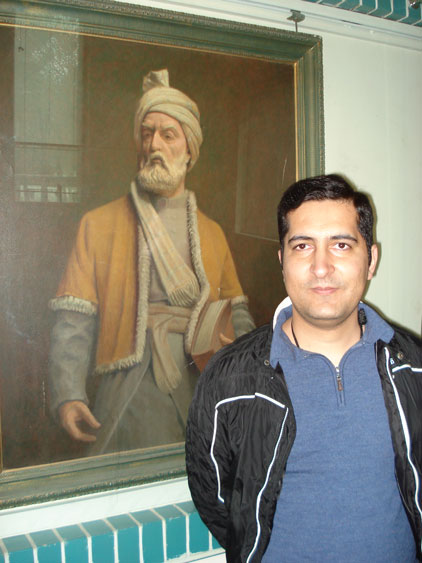
\includegraphics[scale=.5]{Dr_Khaliqi}

\end{figure}

\begin{diagram}[h]
\centering

\includegraphics[scale=.2]{logo}
\caption{دیاگرام تنتبنبلت}
\end{diagram}

\begin{figure}[!ht]
  \centering
  \subfloat[ابوالوفا بوزجانی(ریاضی‌دان و منجم ایرانی)]{\label{sf1}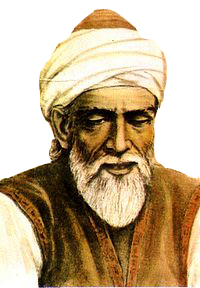
\includegraphics[scale=1.5]{buzjani}}
\quad     \subfloat[دکتر وفا خلیقی(مولف زی‌پرشین)]{\label{sf2}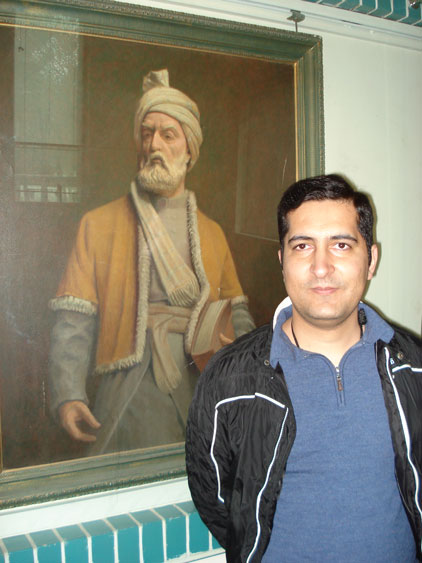
\includegraphics[scale=.26]{Dr_Khaliqi}}\\
    \subfloat[لیزلی لمپارت(مولف لاتک)]{\label{sf3}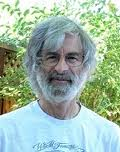
\includegraphics[scale=.9]{LeslieLamport}}
\quad      \subfloat[دونالد کنوث(مولف تک)]{\label{sf4}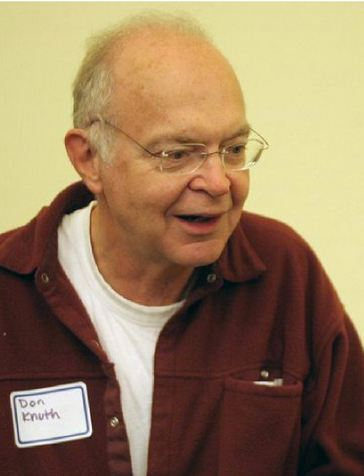
\includegraphics[scale=.29]{knuth}}
  \caption{گذاشتن نمودارها در کنار هم}\label{fi44}
\end{figure}

\ref{sf1}

\clearpage
\subsection{جدول}
به اولین خط جدول توجه ویژه کنید، h و ! دو پارامترهستند که باعث ثابت شدن محیط‌های شناور می‌شوند.

\begin{table}[!ht]
\centering
\caption{می‌توانید در مورد محل عنوان جدول تصمیم‌گیری کنید؟}
\begin{tabular}{lcr}
ردیف &  نام &  نام خانوادگی\\
\hline
$1$ & $2$ & $3$\\
\end{tabular}
\caption{ظاهرامی‌شود.}
\end{table}%pre
\chapter{بسته‌های کاربردی}
\begin{equation}
\begin{cases}
r & \\
r & \\
r & \\
r & \\
\end{cases}
\end{equation}
قبل از شروع بحث لازم است به تراز کردن پاراگراف توجه کنید که به بسته‌ای وابسته نیست و جای تامل بیشتری دارد.

این قسمت هم کاربردی نداردو فقط جنبه زیبایی دارد.

\begin{window}[2,c,\fbox{\hboxR{\bf این یک نمونه است.}},{}]
این یک نمونه است. این یک نمونه است. این یک نمونه است. این یک نمونه است. این یک نمونه است. این یک نمونه است. این یک نمونه است. این یک نمونه است. این یک نمونه است. این یک نمونه است. این یک نمونه است. این یک نمونه است. این یک نمونه است. این یک نمونه است. این یک نمونه است. این یک نمونه است. این یک نمونه است. این یک نمونه است. 
\end{window}


\pagebreak
\diamondpar{
این یک نمونه است. این یک نمونه است. این یک نمونه است. این یک نمونه است. این یک نمونه است. این یک نمونه است. این یک نمونه است. این یک نمونه است. این یک نمونه است. این یک نمونه است. این یک نمونه است. این یک نمونه است. این یک نمونه است. این یک نمونه است. این یک نمونه است. این یک نمونه است. این یک نمونه است. این یک نمونه است. این یک نمونه است. این یک نمونه است. این یک نمونه است. این یک نمونه است. این یک نمونه است. این یک نمونه است. این یک نمونه است. این یک نمونه است. این یک نمونه است. این یک نمونه است. این یک نمونه است. این یک نمونه است. این یک نمونه است. این یک نمونه است. این یک نمونه است. این یک نمونه است. این یک نمونه است. این یک نمونه است. این یک نمونه است. این یک نمونه است. 
}


\pagebreak
\heartpar{
این یک نمونه است. این یک نمونه است. این یک نمونه است. این یک نمونه است. این یک نمونه است. این یک نمونه است. این یک نمونه است. این یک نمونه است. این یک نمونه است. این یک نمونه است. این یک نمونه است. این یک نمونه است. این یک نمونه است. این یک نمونه است. این یک نمونه است. این یک نمونه است. این یک نمونه است. این یک نمونه است. این یک نمونه است. این یک نمونه است. این یک نمونه است. این یک نمونه است. این یک نمونه است. این یک نمونه است. این یک نمونه است. این یک نمونه است. این یک نمونه است. این یک نمونه است. این یک نمونه است. این یک نمونه است. این یک نمونه است. این یک نمونه است. این یک نمونه است. این یک نمونه است. این یک نمونه است. این یک نمونه است. این یک نمونه است. این یک نمونه است. 
}

\pagebreak
\shapepar\nutshape{
این یک نمونه است. این یک نمونه است. این یک نمونه است. این یک نمونه است. این یک نمونه است. این یک نمونه است. این یک نمونه است. این یک نمونه است. این یک نمونه است. این یک نمونه است. این یک نمونه است. این یک نمونه است. این یک نمونه است. این یک نمونه است. این یک نمونه است. این یک نمونه است. این یک نمونه است. این یک نمونه است. این یک نمونه است. این یک نمونه است. این یک نمونه است. این یک نمونه است. این یک نمونه است. این یک نمونه است. این یک نمونه است. این یک نمونه است. این یک نمونه است. این یک نمونه است. این یک نمونه است. این یک نمونه است. این یک نمونه است. این یک نمونه است. این یک نمونه است. این یک نمونه است. این یک نمونه است. این یک نمونه است. این یک نمونه است. این یک نمونه است. 
}

\clearpage
\section{دیاگرام}
%\subsection{بسته \text{pst-node}}
%برای رسم دیاگرام بسته‌های زیادی پیش رو داریم اما از این‌همه شاید بسته ی xy ساده‌ترین راه حل باشد، اما به دلیل این‌که این بسته با بسته ی breqn مشکل دارد، ما  بسته ی pst-node را نیز پیشنهاد می‌کنیم.
%برای نمونه دیاگرام زیر 
%\[
%\begin{psmatrix}
%U \\
%& X \times_Z Y & X \\
%& Y & Z
%\psset{arrows=->,nodesep=3pt}
%\ncline{1,1}{2,2}\tbput{yy}
%\ncline[doubleline=true,linestyle=dashed]{-}{1,1}{2,3}\taput{x}
%\ncline{2,2}{3,2}\tlput{qq}
%\ncline{2,2}{2,3}\tbput{pp}
%\ncline{2,3}{3,3}\tlput{f}
%\ncline{3,2}{3,3}\tbput{g}
%\end{psmatrix}
%\]
%با قطعه کد زیر و فراخوانی بسته pst-node تولید شده است. اگر متوجه نشدید به توضیحات بعدی توجه کنید.
%\begin{LTR}
%\begin{verbatim}
%\[
%\begin{psmatrix}
%U \\
%& X \times_Z Y & X \\
%& Y & Z
%\psset{arrows=->,nodesep=3pt}
%\ncline{1,1}{2,2}\taput{yy}
%\ncline[doubleline=true,linestyle=dashed]{-}{1,1}{2,3}ˆ{x}
%\ncline{2,2}{3,2}\tlput{qq}
%\ncline{2,2}{2,3}\tbput{pp}
%\ncline{2,3}{3,3}\tlput{f}
%\ncline{3,2}{3,3}\tbput{g}
%\end{psmatrix}
%\]
%\end{verbatim}
%\end{LTR}
%اولین و مهم‌ترین چیزی که باید بدانید این است  که همه دیاگرام‌های مورد نظر ما راس ها‌یشان دقیقا می‌تواننددر یک ماتریس واقع بشوند. دراین بسته هر راس با شماره درایه‌ایش در همین ماتریس قابل دسترسی ست.
%
%در مرحله اول توجه داشته باشین که دستورات راباید در یک محیط ریاضی قرار بدهید، اسم محیط در این‌جا \lr{psmatrix} است، راس که کاملا وضع‌شان مشخص است ،شبیه محیط \lr{array} و همه‌ محیط ‌های تراز دار رسم می‌شود. تنها مطلب باقیمانده  این است که برای رسم خطوط از دستور \lr{\bs ncline} استفاده می‌‌شود که جفت آرگومان اولش مختصات راس اول طبق توضیح بالاست و جفت دومش هم راس دومی ست که هر خط ارتباطی(یال) را می‌شودباآن مشخص کرد. حال دستور \lr{\bs psset} را معرفی می‌کنیم که تنظیمات کلی یال‌ها از محل قرار گرفتنش تا رسیدن به دستور دیگری از همین نوع را انجام می‌دهد.
%درپایان برای اندیس‌ها هم اگر یال عمودی باشد برای قرار دادن اندیس در چپ و راستش به ترتیب از \lr{\bs tlput} و \lr{\bs trput}، و اگر هم یال افقی بود برای قرار دادن اندیس در بالا و پایینش به ترتیب از \lr{\bs taput} و \lr{\bs tbput} استفاده می کنیم و خوب در همه این موارد اندیس را به عنوان آرگومان این دستورات قرار می‌دهیم.
%\[
%\begin{psmatrix}
%\pi_1({\mathbb{R}^2}\backslash{Q_{m,i}}) & \pi_1(F(\mathbb{R}^2,m)) & \pi_1(F(\mathbb{R}^2,m-1))\\
%\pi_1({S^2}\backslash{Q_{m,i}}) & \pi_1(B_i) & \pi_1(F(\mathbb{R}^2,m-1))
%\psset{arrows=->, nodesep=3pt}
%\ncline{1,1}{2,1}\trput{f|_*}
%\ncline{1,2}{2,2}\trput{f_*}
%\ncline{1,1}{1,2}\taput{g_{1*}}
%\ncline{1,2}{1,3}\taput{g_{3*}}
%\ncline{2,1}{2,2}\taput{g_{2*}}
%\ncline{2,2}{2,3}\taput{g_{4*}}
%\psset{arrows=-, nodesep=3pt}
%\ncline[offset=3pt]{1,3}{2,3}
%\ncline[offset=-3pt]{1,3}{2,3}
%\end{psmatrix}
%\]
%
%\[
%\begin{psmatrix}
%B & C \\
%A & \\
%\bar{A}^{(S)}
%\psset{arrows=->, nodesep=3pt}
%\ncline{1,1}{1,2}\taput{h}
%\ncline{1,1}{2,1}\tlput{f}
%\ncline[linestyle=dashed]{1,2}{2,1}\trput{g}
%\ncline[linestyle=dashed]{1,2}{3,1}\trput{k}
%\ncline{2,1}{3,1}\tlput{\varphi}
%\ncarc[arcangle=50]{3,1}{2,1}\tlput{l}
%\end{psmatrix}
%\]
%
%\[
%\begin{psmatrix}
%& C & \\
%A & B & B\sqcup_A B
%\psset{arrows=->, nodesep=3pt}
%\ncline{1,2}{2,1}\tlput{\bar{f}}
%\ncline{1,2}{2,2}\trput{f}
%\ncline{2,1}{2,2}\tbput{h}
%\ncline[offset=3pt]{2,2}{2,3}\taput{g_1}
%\ncline[offset=-3pt]{2,2}{2,3}\tbput{g_2}
%\end{psmatrix}
%\]
%
%اما هنر این بسته به همین‌جا هم ختم نمی‌شود.
%
%\[
%\begin{pmatrix}
%& x_{11} & x_{12} & \dots & x_{1p} & \rdelim\}{4}{3cm}[some text]\\
%\ldelim[{5}{1cm}[text] & x_{21} & x_{22} & \dots & x_{2p} \\
%& \vdots\\
%& x_{n_1 1}& x_{n_1 2} & \dots & x_{n_1 p}\\
%& x_{n_1+1,1}&x_{n_1+1,2} & \dots & x_{n_1+1, p} &
%\rdelim\}{3}{3cm}[some more text]\\
%& \vdots\\
%& x_{n_1+n_2, 1} & x_{n_1+n_2,2} & \dots & x_{n_1+n_2,p}\\
%& \vdots \\
%\end{pmatrix}
%\]


\subsection{بسته \text{xy}}

\[
\xymatrix{
A \ar@<.5ex>[r]^f\ar@<-.5ex>[r]_g & B\ar[d]_{c'}\ar[r]^c & C\ar[ld]^{\overline{c}} \\
& C' & 
}
\]

\[
\xymatrix{
 & X\ar@<.5ex>[r]^{f}\ar@<-.5ex>[r]_{g} & Y\\
A \ar[r]_{u_k\qquad}\ar[ru]^k& \mathop{\sqcup}\limits_{k\in pos_S(A,X)}A\ar@{-->}_h[u]
}
\]

\[
\xymatrix{
\ar[dd]_{g\circ f} & _T\!B \ar[d]_{f}\ar[r] & _T\! pos(A,B)\ar[d]^{_T\! pos(A,f)} & \ar[dd]^{_T\! pos(A,g\circ f)}\\
& _T\!C\ar[r]\ar[d]_{g} & _T\! pos(A,C)\ar[d]^{_T\! pos(A,g)} & \\
& _T\!D\ar[r] \ar[r] & _T\! pos(A,D) &
}
\]

\section{رسم فلوچارت با \text{tikz}}
\begin{center}
\begin{tikzpicture}
[auto,
decision/.style={diamond, draw=blue, thick, fill=blue!20,
text width=4.5em,align=flush center,
inner sep=1pt},
block/.style ={rectangle, draw=blue, thick, fill=blue!20,
text width=5em,align=center, rounded corners,
minimum height=4em},
line/.style ={draw, thick, -latex',shorten >=2pt},
cloud/.style ={draw=red, thick, ellipse,fill=red!20,
minimum height=2em}]
\matrix [column sep=5mm,row sep=7mm]
{
% row 1
\node [cloud] (expert) {expert}; &
\node [block] (init) {initialize model}; &
\node [cloud] (system) {system}; \\
% row 2
& \node [block] (identify) {identify candidate model}; & \\
% row 3
\node [block] (update) {update model}; &
\node [block] (evaluate) {evaluate candidate models}; & \\
% row 4
& \node [decision] (decide) {is best candidate}; & \\
% row 5
& \node [block] (stop) {stop}; & \\
};
\begin{scope}[every path/.style=line]
\path (init) -- (identify);
\path (identify) -- (evaluate);
\path (evaluate) -- (decide);
\path (update) |- (identify);
\path (decide) -| node [near start] {yes} (update);
\path (decide) -- node [midway] {no} (stop);
\path [dashed] (expert) -- (init);
\path [dashed] (system) -- (init);
\path [dashed] (system) |- (evaluate);
\end{scope}
\end{tikzpicture}
\end{center}



\section{کدهای برنامه‌نویسی}

\begin{latin}
\lstinputlisting[lineskip=0.001cm,breaklines=true,numbers=left,language=Matlab, basicstyle=\ttfamily\small, numberstyle=\footnotesize , numbersep=10pt, captionpos=b, frame=single, breakatwhitespace=false]{code/matlab.m}
\end{latin}

\begin{latin}
\lstinputlisting[lineskip=0.008cm,breaklines=true,numbers=left,language=c++, basicstyle=\ttfamily\scriptsize, numberstyle=\footnotesize , commentstyle=\footnotesize\color{green}, numbersep=10pt, captionpos=b, frame=single, breakatwhitespace=false]{code/cpp.cpp}
\end{latin}

\section{رسم نمودار}
\subsection{رسم نمودارهای قطبی}
برای رسم این دسته از نمودارها از بسته \lr{pst-plot} استفاده می‌کنیم.
%\begin{figure}[!ht]
%\centering
%\scalebox{.5} % Change this value to rescale the drawing.
%{
%\begin{pspicture}(3,3)(-3,-3)
% \psaxes{<->}(0,0)(3,3)(-3,-3)
% \psplot[polarplot,algebraic=true,linecolor=yellow,linewidth=1pt,
% plotpoints=2000]{0}{TwoPi 4 mul}{2*(sin(2*x))}
%  \psplot[polarplot,algebraic=true,linecolor=red,linewidth=1pt,
% plotpoints=2000]{0}{TwoPi 4 mul}{2*(cos(2*x))}
% \end{pspicture} 
% }
%\end{figure}
%
%\begin{figure}[!ht]
%\centering
%\scalebox{.5} % Change this value to rescale the drawing.
%{
%\begin{pspicture}(3,3)(-3,-5)
% \psaxes{<->}(0,0)(3,3)(-3,-5)
% \psplot[polarplot,algebraic=true,linecolor=blue,linewidth=1pt,
% plotpoints=2000]{0}{TwoPi 4 mul}{2}
%  \psplot[polarplot,algebraic=true,linecolor=green,linewidth=1pt,
% plotpoints=2000]{0}{TwoPi 4 mul}{2*(1-sin(x))}
% \end{pspicture} 
% }
%\end{figure}
\subsection{نمودارهای دکارتی با استفاده از بسته tikz}
می دانید 
همیشه برای کار با بسته ی  tikz یک محور مختصات مجازی داریم.
پس سریع یک  مبدا هر جا که می‌خواهید در نظر بگیرید و هر چیزی را که می‌خواهید نسبت به آن تعیین موقعیت کنید.

تابلوی جادویی‌ای که باید در آن شروع به کشیدن کنید، چیست؟

\lstset{framexleftmargin=5mm, frame=shadowbox, rulesepcolor=\color{blue}, language=Tex}
\begin{latin}
\begin{lstlisting}[frame=trBL]
\begin{tikzpicture}

\end{tikzpicture}
\end{lstlisting}
\end{latin}
اما برای این‌که شروع به رسم کنید، باید بدانید که از چه دستوراتی برای رسم در این محیط می‌توانید استفاده کنید.

ضمنا لازم به ذکر است که هر خط دستور که می‌نویسید باید با ;(سمیکولن) آن‌را تمام کنید.

\begin{description}
\item[draw]
برای اشکال پایه که با دستور فوق می‌خواهید رسم کنید به دو جفت مختصات نیاز دارید که بین آن‌ها نوع شکل را مشخص می‌کنید، البته دقیق .بعد از دستور هم تنظیماتی اختیاری وجود دارند که با آن‌ها آشنا خواهید شد.

\lstset{framexleftmargin=5mm, frame=shadowbox, numbers=left, rulesepcolor=\color{blue}, language=Tex}
\begin{latin}
\begin{lstlisting}[frame=trBL]
\begin{tikzpicture}
\draw[color=cm1, ] (x1, y1) fig (x2, y2);
\draw[step=.5cm,gray,very thin] (x1, y1) grid (x2, y2);
\clip[draw] (x1, y1) fig (x2, y2);
\end{tikzpicture}
\end{lstlisting}
\end{latin}

در دستور فوق در جفت پرانتزها مختصات را قرار می‌دهیم که برای مستطیل اولی مختصات راس چپ‌ِ پایین و دومی مختصات راس راستِ بالا است و در دایره اولی مختصات مرکز و دومی شعاع است. بین دو پرانتز به جای fig می‌توانید از اشکال --(خط ساده)، circle (دایره)، rectangle (مستطیل) و arc (زاویه) استفاده کنید. برای تنظیمات اختیاری هم می‌توانید با مطالعه ی ‌‌راهنمای tikz بیشتر آشنا شوید(هر چند که ما هم چندتا از آن‌ها را معرفی می‌کنیم.

برای رسم شبکه در زمینه شکل از دستور grid استفاده می‌شود که خط سوم کد فوق شامل این دستور است.

برای گرفتن یک نمای خاص با هر یک از شکل‌های یاد شده از دستور کلیپ می‌توان استفاده کرد(مطابق خط چهارم کد فوق).

ما همه چیز را نگفتیم اگر می‌خواهید بیشتر بدانید تا حد امکان به کد زیر و خروجی آن دقت کنید.

\lstset{framexleftmargin=5mm, frame=shadowbox, numbers=left, rulesepcolor=\color{blue}, language=Tex}
\begin{latin}
\begin{lstlisting}[frame=trBL]
\begin{center}
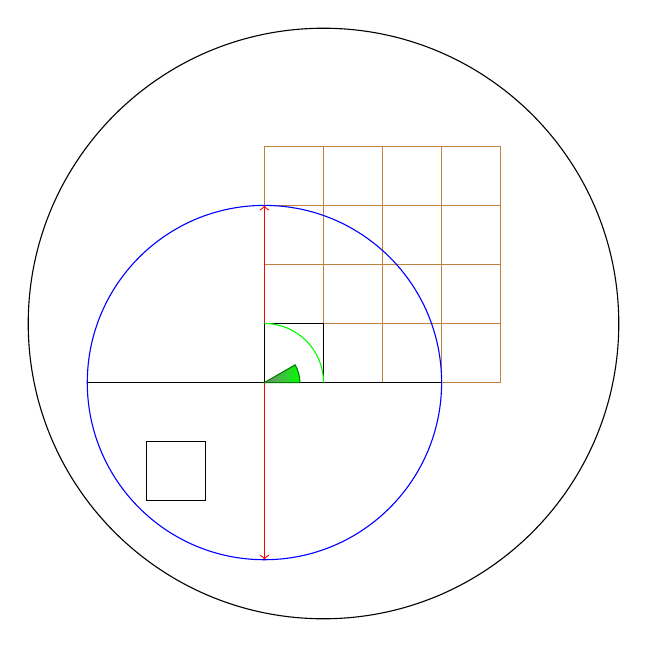
\begin{tikzpicture}[scale=1.5]
\clip[draw] (.5,.5) circle (2.5);
\draw[step=.5cm, gray,color=brown] (0,0) grid (2,2);
\draw (-1.5,0) -- (1.5,0);
\draw [color=red,<->] (0,-1.5) -- (0,1.5);
\draw[color=blue] (0,0) circle (1.5cm);
\draw (0,0) rectangle (0.5,0.5);
\draw (-0.5,-0.5) rectangle (-1,-1);
\draw [color=green] (5mm,0mm) arc (0:90:5mm);
\shadedraw[left color=gray,right color=green, draw=
green!50!black](0,0) -- (3mm,0mm) arc (0:30:3mm) -- cycle;
\end{tikzpicture}
\end{center}
\end{lstlisting}
\end{latin}


\begin{center}
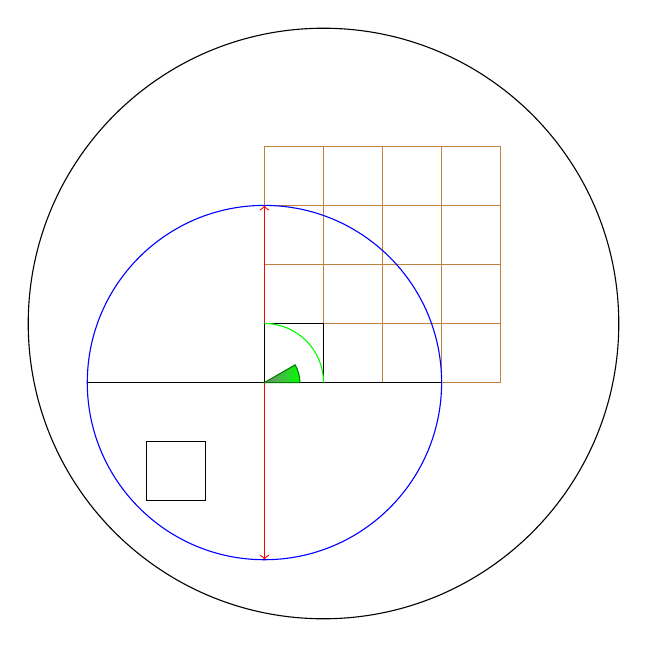
\begin{tikzpicture}[scale=1.5]
\clip[draw] (.5,.5) circle (2.5);
\draw[step=.5cm, gray,color=brown] (0,0) grid (2,2);
\draw (-1.5,0) -- (1.5,0);
\draw [color=red,<->] (0,-1.5) -- (0,1.5);
\draw[color=blue] (0,0) circle (1.5cm);
\draw (0,0) rectangle (0.5,0.5);
\draw (-0.5,-0.5) rectangle (-1,-1);
\draw [color=green] (5mm,0mm) arc (0:90:5mm);
\shadedraw[left color=gray,right color=green, draw=green!50!black](0,0) -- (3mm,0mm) arc (0:30:3mm) -- cycle;
\end{tikzpicture}
\end{center}

اما این همه‌ی هنر این دستور نیست شما تقریبا هر نمودار در فضای ۲بعدی و مختصات دکارتی رامی‌توانید با دستور plot در دستور draw بکشید، برای نمونه می‌توانید دو تا کد زیر و خروجی‌شان را ملاحظه کنید.\footnote{تنها چیزی که لازم است یادآوری کنم این است که دقت کنید هر خط با سمیکولن تمام می‌شود پس اگرانتهای خطی خالی ست بدانید که ادامه دستور در خط بعد آمده، این رااز این بابت گفتم که بتوانید کد رابرای خودتان تشریح کنید}
\begin{center}
\begin{tikzpicture}[scale=.6]
\draw[->] (-7,0) -- (7,0) node[right] {$x$};
\draw[->] (0,-5) -- (0,7) node[above] {$y$};
\draw[color=blue] plot[domain=-6.5:-1.18, samples=70, smooth] (\x, {((\x)^2+1)/((\x)^2-1)}) node[right] {};
\draw[color=blue] plot[domain=1.18:6.5, samples=70, smooth] (\x, {((\x)^2+1)/((\x)^2-1)}) node[right] {};
\draw[color=blue] plot[domain=-.8:.8, samples=70, smooth] (\x, {((\x)^2+1)/((\x)^2-1)}) node[right] {};
\draw[color=blue] plot[domain=-6.5:6.5] (\x, { 1}) node[right] {};
\draw[blue] (1,-4.5) -- (1,6.5) node[above] {};
\draw[blue] (-1,-4.5) -- (-1,6.5) node[above] {};
\fill[blue] (0,-1) circle (.1) (2,1.67) circle (.1) (-2,1.67) circle (.1) (.5,-1.67) circle (.1) (-.5,-1.67) circle (.1) (0,1) circle (.1);
\end{tikzpicture}
\end{center}
\lstset{framexleftmargin=5mm, frame=shadowbox, numbers=left, rulesepcolor=\color{blue}, language=Tex}
\begin{latin}
\begin{lstlisting}[frame=trBL]
\begin{center}
\begin{tikzpicture}[scale=.8]
\draw[->] (-7,0) -- (7,0) node[right] {$x$};
\draw[->] (0,-5) -- (0,7) node[above] {$y$};
\draw[color=blue] plot[domain=-6.5:-1.18, samples=70, smooth] 
(\x, {((\x)^2+1)/((\x)^2-1)}) node[right] {};
\draw[color=blue] plot[domain=1.18:6.5, samples=70, smooth] 
(\x, {((\x)^2+1)/((\x)^2-1)}) node[right] {};
\draw[color=blue] plot[domain=-.8:.8, samples=70, smooth] 
(\x, {((\x)^2+1)/((\x)^2-1)}) node[right] {};
\draw[color=blue] plot[domain=-6.5:6.5] 
(\x,{1}) node[right] {};
\draw[blue] (1,-4.5) -- (1,6.5) node[above] {};
\draw[blue] (-1,-4.5) -- (-1,6.5) node[above] {};
\fill[blue] (0,-1) circle (.1) (2,1.67) circle (.1) 
(-2,1.67) circle (.1) (.5,-1.67) circle (.1) 
(-.5,-1.67) circle (.1) (0,1) circle (.1);
\end{tikzpicture}
\end{center}
\end{lstlisting}
\end{latin}
نمونه‌ی دیگر یک نمودار مثلثاتی ست که تنها یک تفاوت کوچک برای رسمش هست که مختصات رابه رادیان تبدیل می‌کند\footnote{واقعا فکر می‌کنید اگر با گذاشتن کد و خروجی آن را هم می‌گفتم تا زحمت چک کردن هم به خودتان ندهید کار خوبی بود؟!}.
\begin{center}
\begin{tikzpicture}[scale=1, domain=-3.3:3.3]
\draw[->] (-3.5,0) -- (3.5,0) node[right] {$x$};
\draw[->] (0,-5) -- (0,5) node[above] {$y$};
\draw[color=blue] plot[ samples=100, smooth]  (\x, {3*cos(2*\x r)}) node[right] {};
\fill[blue] (-3.14,3) circle (.08) (-1.57,-3) circle (.08) (-.775,0) circle (.08) (0,3) circle (.08) (.775,0) circle (.08) (1.57,-3) circle (.08) (3.14,3) circle (.08);
\draw[blue,dashed] (-1.57,0) -- (-1.57,-3) -- (1.57,-3) -- (1.57,0) (-3.14,0) --(-3.14,3)--(3.14,3)--(3.14,0);
\foreach \x/\xtext in {-3.14/-\pi, -1.57/-\frac{\pi}{2}, -.775/-\frac{\pi}{4}, 0/0, .775/\frac{\pi}{4}, 1.57/\frac{\pi}{2}, 3.14/\pi}
\draw[shift={(\x,0)}] (0pt,0pt) -- (0pt,0pt) node[below] {$\xtext$};
\end{tikzpicture}
\end{center}
\lstset{framexleftmargin=5mm, frame=shadowbox, numbers=left, rulesepcolor=\color{blue}, language=Tex}
\begin{latin}
\begin{lstlisting}[frame=trBL]
\begin{center}
\begin{tikzpicture}[scale=1, domain=-3.3:3.3]
\draw[->] (-3.5,0) -- (3.5,0) node[right] {$x$};
\draw[->] (0,-5) -- (0,5) node[above] {$y$};
\draw[color=blue] plot[ samples=100, smooth] 
(\x, {3*cos(2*\x r)}) node[right] {};
\fill[blue] (-3.14,3) circle (.08) (-1.57,-3) circle (.08)
 (-.775,0) circle (.08) (0,3) circle (.08) 
 (.775,0) circle (.08) (1.57,-3) circle (.08) 
 (3.14,3) circle (.08);
\draw[blue,dashed] (-1.57,0) -- (-1.57,-3) -- (1.57,-3)
 -- (1.57,0) (-3.14,0) --(-3.14,3)--(3.14,3)--(3.14,0);
\foreach \x/\xtext in {-3.14/-\pi, -1.57/-\frac{\pi}{2},
 -.775/-\frac{\pi}{4}, 0/0, .775/\frac{\pi}{4},
  1.57/\frac{\pi}{2}, 3.14/\pi}
\draw[shift={(\x,0)}] (0pt,0pt) -- (0pt,0pt)
 node[below] {$\xtext$};
\end{tikzpicture}
\end{center}
\end{lstlisting}
\end{latin}

\item[fill]
دستور fill هم مشابه دستور draw است، فقط این‌که طبیعتا از آن انتظار داریم همه‌ی اشکال را تو پر بکشد.\footnote{فکر می‌کنم تا همین جا کافی باشد اگر بیشتر از این نمونه خواستید، و از راهنمای tikz نتوانستید استفاده کنید با ما تماس بگیرید، تا در حد توان تجربیات‌مان را تقدیم‌تان کنیم.} البته کاربردش را هم می‌توانید در کدهای بالا ببینید.
\end{description}

\begin{center}
\begin{tikzpicture}[scale=1]
\draw[blue] (.5,0) rectangle (7,4) node[right] {\rl{دانشکده}};
\draw[blue] (2.5,2) circle (1.5) node[] {$A$\ \rl{حسابداری}};
\draw[blue] (5,2) circle (1.5) node[] {$B$\ \rl{مدیریت}};
\end{tikzpicture}

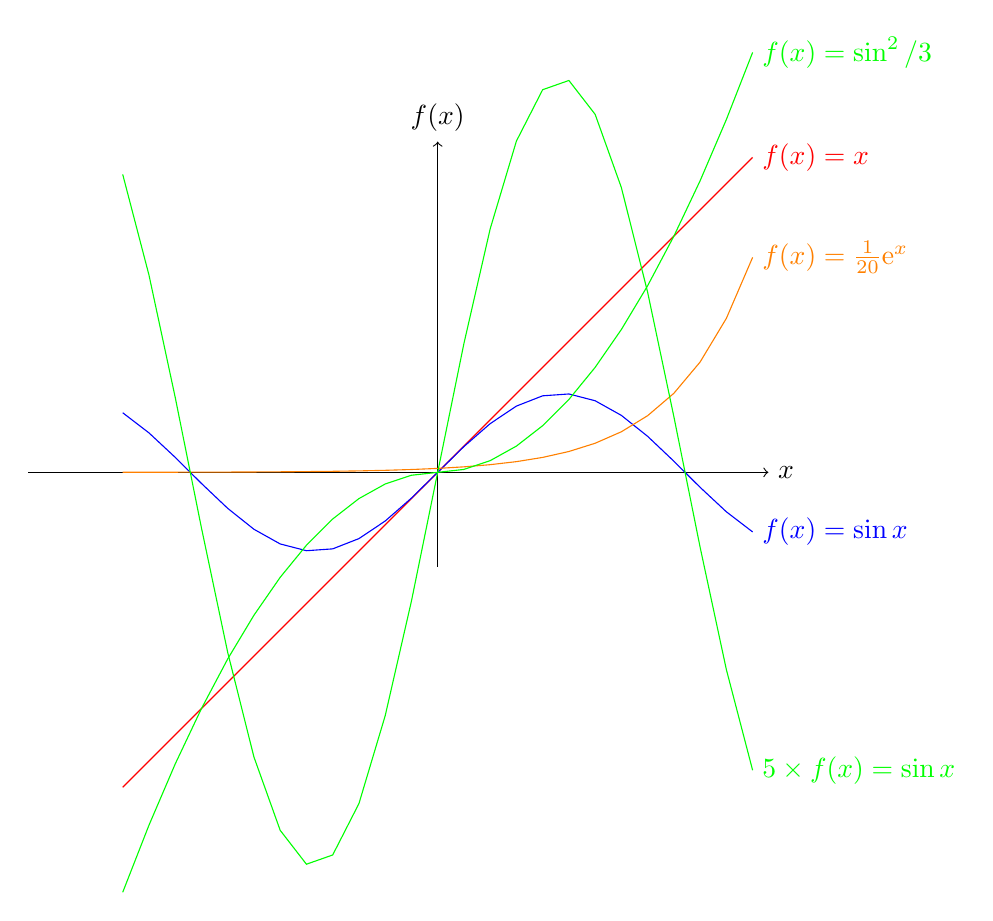
\begin{tikzpicture}[domain=-4:4]
%\draw[very thin,color=gray] (-5,-1.1) grid (9,5);
\draw[->] (-5.2,0) -- (4.2,0) node[right] {$x$};
\draw[->] (0,-1.2) -- (0,4.2) node[above] {$f(x)$};
\draw[color=red] plot (\x,\x) node[right] {$f(x) =x$};
\draw[color=blue] plot (\x,{sin(\x r)}) node[right] {$f(x) = \sin x$};
\draw[color=orange] plot (\x,{0.05*exp(\x)}) node[right] {$f(x) = \frac{1}{20} \mathrm e^x$};
\draw[color=green] plot (\x,{5*sin(\x r)}) node[right] {$5\times f(x) = \sin x$};
\draw[color=green] plot (\x,{(\x^2)/3}) node[right] {$f(x) = \sin^2/ 3$};
\end{tikzpicture}
\end{center}

%\section{بسته tabvar برای رسم جداول تعیین علامت}
%در این قسمت فقط می‌تونید نمونه‌ها رو ببینید، چون واقعا چیز زیادی برا گفتن نداره.
%
%\[\begin{tabvar}{ C|CCCCCCCC} 
%x &-\infty & &1 & &\frac{5}{3}& & +\infty
%\\ \hline
%f'(x)& &+& \barre{0} &- &\barre{0} &+ & &
%\\ \hline
%f(x) &  &\niveau{2}{2}\text{صعودی} &\niveau{0}{ 1}\barre{\text{ماکزیمم}}&\niveau{2}{2}\text{نزولی}&\niveau{0}{1}\barre{\text{مینیمم}}
% &\niveau{2}{2}\text{صعودی}&
%\end{tabvar}\]
%
%\[\begin{tabvar}{C|CCCCCCCCC} 
%x &-\infty & &-1& &0& &+1 & &+\infty 
%\\ \hline
%f'(x) & &+&\barre{0} &-&\dbarre{}&-&\barre{0}&+&
%\\ \hline
%f''(x)& &-&\barre{}&-&\dbarre{}&+&\barre{}&+&
%\\ \hline
%\niveau{2}{2}\TVcenter{f(x)}& &\niveau{2}{2}\TVcenter{\text{صعودی محدب}}&\niveau{0}{1}\barre{\text{ماکزیمم}}&\niveau{2}{2}\TVcenter{\text{نزولی محدب}}&\dbarre{}&\TVcenter{\text{نزولی مقعر}}
%&\niveau{0}{1}\barre{\text{مینیمم}}&\niveau{2}{2}\TVcenter{\text{صعودی مقعر}}&
%\end{tabvar}\]
%
%\[\begin{tabvar}{C|CCCCCCCCC} 
%x &-\infty & &-1& &1& &5& &+\infty \\ \hline
%(1+x)^2& &+&\barre{0}&+&\barre{}&+&\barre{}&+& \\ \hline
%1-x& &+&\barre{}&+&\barre{0}&-&\barre{}&-&\\ \hline
%x-5& & -&\barre{}&-&\barre{}&-&\barre{0}&+&\\ \hline
%f'(x) & &-&\barre{0} &-&\barre{0}&+&\barre{0}&-&\\ \hline
%\niveau{3}{3}\TVcenter{f(x)}& &\decroit &\niveau{0}{2}\barre{}&\niveau{3}{3}\decroit &
%\niveau{0}{2}\barre{\text{مینیمم}}&\niveau{3}{3}\TVcenter{\croit} & \niveau{0}{2}\barre{\text{ماکزیمم}}&\niveau{3}{3}{\decroit} &
%\end{tabvar}\]


\section{رسم گراف}
%\begin{figure}[!ht]
%\centering
%\scalebox{.7}
%{
%\begin{pspicture}(0,0)
%\pscircle[linewidth=.015,dimen=outer](0,0){.4}
%\rput(0,0){$1$}
%\psline[linewidth=.01cm,arrowsize=.1cm,arrowlength=1.5,arrowinset=.2]{-}(-.255,-.255)(-1.15,-1.1)
%\rput(-1.2,-.6){$u_3=0$}
%\psline[linewidth=.01cm,arrowsize=.1cm,arrowlength=1.5,arrowinset=.2]{-}(.26,-.255)(1.2,-1.1)
%\rput(1.6,-.6){$g_3=0$}
%\pscircle[linewidth=.015,dimen=outer](1.4,-1.4){.4}
%\rput(1.4,-1.4){$4$}
%\pscircle[linewidth=.015,dimen=outer](-1.4,-1.4){.4}
%\rput(-1.4,-1.4){$0$}
%\psline[linewidth=.01cm,arrowsize=.1cm,arrowlength=1.5,arrowinset=.2]{-}(-1.65,-1.67)(-2.52,-2.52)
%\pscircle[linewidth=.015,dimen=outer](-2.8,-2.8){.4}
%\rput(-2.8,-2.8){$2$}
%\rput(-2.5,-2){$u_2=0$}
%\psline[linewidth=.01cm,arrowsize=.1cm,arrowlength=1.5,arrowinset=.2]{-}(-2.35,-3.37)(-3.35,-3.37)
%\psline[linewidth=.01cm,arrowsize=.1cm,arrowlength=1.5,arrowinset=.2]{-}(-1.1,-1.65)(-.23,-2.52)
%\rput(0,-2){$g_2=0$}
%\pscircle[linewidth=.015,dimen=outer](0,-2.8){.4}
%\rput(0,-2.8){$3$}
%\end{pspicture} 
%}
%\end{figure}


%\begin{center}
%\begin{tikzpicture}
%\GraphInit[vstyle=Shade]
%\SetVertexNoLabel
%\grTriangularGrid[RA=1,form=2]{6}%
%\end{tikzpicture}
%\end{center}


%\begin{center}
%\begin{tikzpicture}
%\GraphInit[vstyle=Shade]
%\SetVertexLabel
%\grTriangularGrid[prefix=G,Math,RA=1.2]{8}%
%\end{tikzpicture}
%\end{center}
%
%\begin{center}
%\begin{tikzpicture}%
%\GraphInit[vstyle=Art]
%\SetGraphArtColor{black!50}{darkgray}
%\tikzset{VertexStyle/.append style = {
%minimum size = 2pt}}
%\grLCF[RA=3]{1,-3}{4}%
%\end{tikzpicture}
%\end{center}

%\begin{tikzpicture}[scale=1.75]
%\GraphInit[vstyle=Art]
%\Vertex{A}
%\Vertex[x=4,y=0]{B}
%\Vertex[x=1,y=2]{C}
%\Edge[style={bend left}](B)(A)
%\Edges(A,B,C,A)
%\end{tikzpicture}

%\begin{center}
%\begin{tikzpicture}
%\useasboundingbox (-1,-1) rectangle (11,11);
%\tikzset{VertexStyle/.style = {shape = circle,
%ball color = orange,
%text = black,
%inner sep = 2pt,
%outer sep = 0pt,
%minimum size = 24 pt}}
%\tikzset{EdgeStyle/.style = {thick,
%double = orange,
%double distance = 1pt}}
%\tikzset{LabelStyle/.style = {draw,
%fill = yellow,
%text = red}}
%\node[VertexStyle](A){A};
%\node[VertexStyle,right= of A](B){B};
%\node[VertexStyle,right= of B](C){C};
%\node[VertexStyle,above= 7 cm of B](D){D};
%\draw[EdgeStyle](B) to node[LabelStyle]{1} (D) ;
%\tikzset{EdgeStyle/.append style = {bend left}}
%\draw[EdgeStyle](A) to node[LabelStyle]{2} (B);
%\draw[EdgeStyle](B) to node[LabelStyle]{3} (A);
%\draw[EdgeStyle](B) to node[LabelStyle]{4} (C);
%\draw[EdgeStyle](C) to node[LabelStyle]{5} (B);
%\draw[EdgeStyle](A) to node[LabelStyle]{6} (D);
%\draw[EdgeStyle](D) to node[LabelStyle]{7} (C);
%\end{tikzpicture}
%\end{center}

%\begin{tikzpicture}
%\SetGraphUnit{4}
%\Vertex{a}
%\EA(a){b}
%\SO[unit=2](a){c}
%\EA(c){d}
%{\SetGraphUnit{2}
%\SO(c){e}}
%\EA(e){f}
%\Edge(a)(b)
%\tikzset{EdgeStyle/.style = {-,bend left}}
%\Edge(c)(d)
%\tikzset{EdgeStyle/.style = {<->,bend right=90}}
%\Edge(e)(f)
%\end{tikzpicture}

%\begin{tikzpicture}
%\SetVertexNormal[Shape = circle,
%FillColor = orange,
%LineWidth = 2pt]
%\SetUpEdge[lw = 1.5pt,
%color = black,
%labelcolor = white,
%labeltext = red,
%labelstyle = {sloped,draw,text=blue}]
%\Vertex[x=0 ,y=0]{K}
%\Vertex[x=0 ,y=2]{F}
%\Vertex[x=-1,y=4]{D}
%\Vertex[x=3 ,y=7]{H}
%\Vertex[x=8 ,y=5]{B}
%\Vertex[x=9 ,y=2]{N}
%\Vertex[x=5 ,y=0]{M}
%\Vertex[x=3 ,y=1]{S}
%\tikzset{EdgeStyle/.append style = {bend left}}
%\Edge[label = $120$](K)(F)
%\Edge[label = $650$](H)(S)
%\Edge[label = $780$](H)(M)
%\Edge[label = $490$](D)(B)
%\Edge[label = $600$](D)(M)
%\Edge[label = $580$](B)(M)
%\Edge[label = $600$](H)(N)
%\Edge[label = $490$](F)(H)
%\tikzset{EdgeStyle/.append style = {bend right}}
%\Edge[label = $630$](S)(B)
%\Edge[label = $210$](S)(N)
%\Edge[label = $230$](S)(M)
%\end{tikzpicture}

%\begin{tikzpicture}
%\GraphInit[vstyle=Shade]
%\SetGraphUnit{3}
%\Vertex{e}
%\NOEA(e){f}\SOEA(e){d}
%\SOEA(f){h}\NOWE(f){g}
%\WE(g){c} \SOWE(e){a} \SOWE(c){b}
%\tikzstyle{LabelStyle}=[fill=white]
%\tikzstyle{EdgeStyle}=[color=red]
%\Edge[label=$3$](a)(b)
%\Edge[label=$11$](a)(c)
%\Edge[label=$6$](a)(e)
%\Edge[label=$17$](a)(d)
%\Edge[style={pos=.25},label=$20$](a)(g)
%\Edge[label=$5$](c)(b)
%\Edge[label=$6$](c)(e)
%\Edge[label=$7$](c)(g)
%\Edge[label=$7$](f)(e)
%\Edge[label=$3$](d)(e)
%\Edge[label=$9$](d)(h)
%\Edge[label=$6$](g)(e)
%\Edge[style={bend left,out=45,in=135},label=$11$](g)(h)
%\Edge[label=$4$](f)(h)
%\end{tikzpicture}


%\begin{tikzpicture}
%\SetUpEdge[lw = 1.5pt,
%color = orange,
%labelcolor = gray!30,
%labelstyle = {draw}]
%\SetGraphUnit{3}
%\GraphInit[vstyle=Normal]
%\Vertex{P}
%\NOEA(P){B}
%\SOEA(P){M}
%\NOEA(B){D}
%\SOEA(B){C}
%\SOEA(C){L}
%\tikzset{EdgeStyle/.style={->}}
%\Edge[label=$3$](C)(B)
%\Edge[label=$10$](D)(B)
%\Edge[label=$10$](L)(M)
%\Edge[label=$10$](B)(P)
%\tikzset{EdgeStyle/.style={<->}}
%\Edge[label=$4$](P)(M)
%\Edge[label=$9$](C)(M)
%\Edge[label=$4$](C)(L)
%\Edge[label=$5$](C)(D)
%\Edge[label=$10$](B)(M)
%\tikzset{EdgeStyle/.style={<->,relative=false,in=0,out=60}}
%\Edge[label=$11$](L)(D)
%\end{tikzpicture}


\section{الگوریتم}
%\begin{algorithm}[!ht]
% \SetAlgoLined
%\caption{الگوریتم افزایش دوگان.} \label{alg:dualascent}
%برای هر $j$ اندیس $k(j)$ را به صورت زیر تعریف کنید 
%\[
%k(j) = \min\{k\;:\; v_j\leq c_j^k \}.
%\]
%اگر $v_j = c_j^{k(j)}$ آنگاه قرار دهید $k(j) = k(j)+1$. 
%\\
%
%قرار دهید $\text{improvement=true}$.
%\\
%\While{($\text{improvement=true}$)}{
%	قرار دهید 	$\text{improvement=false}$ . 
%	\\
%	\ForEach{$j\in J^+$}{
%قرار دهید $\Delta_j = \min_{i\in I} \{ \rho_i(v) \;:\; v_j-c_{ij}\geq 0 \}$.
%\\
%		\If{$\Delta_j> c_j^{k(j)} -v_j$}{
% قرار دهید $\Delta_j = c_j^{k(j)} -v_j$  .
%\\
%	 					$\text{improvement=true}$.
%	\\
%متغیر $k(j)$ را یک واحد افزایش دهید.
%\\
%            }
%					$v_j$
% را به اندازه‌ی $\Delta_j$ افزایش دهید. (این کار موجب می‌شود که برای هر $i$،  $\rho_i(v)$ به اندازه‌ی $\Delta_j$ کم شود.)
% \\
% }
%} %ENDWHILE
%\end{algorithm}

\renewcommand{\algorithmicif}{\textbf{اگر}}
\renewcommand{\algorithmicthen}{\textbf{آنگاه}}
\renewcommand{\algorithmicelse}{\textbf{وگرنه}}
\renewcommand{\algorithmicprint}{\textbf{چاپ کن}}
\begin{algorithm}[!ht]
\caption{الگوریتم هم‌رنگ‌سازی چندبانده.} \label{alg:multibandblending}
\begin{algorithmic}[1]
\REQUIRE تصاویر $A$ و $B$.\\
\ENSURE تصویر $S$ حاصل از  نیمه‌ی سمت چپ $A$ و نیمه‌ی سمت راست $B$
  \STATE هرمهای لاپلاسین $LA,LB$ از تصاویر $A,B$ ساخته می‌شوند.
  \STATE هرم لاپلاسین سومی به نام $LS$ با کپی کردن نیمه‌های سمت چپ $LA$ و سمت راست $LB$ ساخته می‌شود.
  \STATE تصویر نهایی $S$ با گسترش هر سطح هرم $LS$ و جمع آن با سطح بعدی حاصل خواهد شد.   
  \IF{$mod(a,2)==0$}
  \PRINT $a$ زوج است.
  \ELSE 
  \PRINT $a$ فرد است.  
\ENDIF
\end{algorithmic}
\end{algorithm}


%\renewcommand{\algorithmicif}{\textbf{اگر}}
%\renewcommand{\algorithmicthen}{\textbf{آنگاه}}
%\renewcommand{\algorithmicelse}{\textbf{وگرنه}}
%\renewcommand{\algorithmicprint}{\textbf{چاپ کن}}
\begin{algorithm}[!ht]
\caption{الگوریتم هم‌رنگ‌سازی چندبانده.} \label{alg:multibandblending}
\begin{algorithmic}[1]
\REQUIRE تصاویر $A$ و $B$.\\
\ENSURE تصویر $S$ حاصل از  نیمه‌ی سمت چپ $A$ و نیمه‌ی سمت راست $B$
  \STATE هرمهای لاپلاسین $LA,LB$ از تصاویر $A,B$ ساخته می‌شوند.
  \STATE هرم لاپلاسین سومی به نام $LS$ با کپی کردن نیمه‌های سمت چپ $LA$ و سمت راست $LB$ ساخته می‌شود.
  \STATE تصویر نهایی $S$ با گسترش هر سطح هرم $LS$ و جمع آن با سطح بعدی حاصل خواهد شد.   
  \IF{$mod(a,2)==0$}
  \PRINT $a$ زوج است.
  \ELSE 
  \PRINT $a$ فرد است.  
\ENDIF
\end{algorithmic}
\end{algorithm}

\begin{algorithm}[!ht]
\caption{الگوریتم برنامه شرالی-آدامز برای دستگاه‌های تساوی}\label{sh-ad}
\begin{algorithmic}[1]
\item[(*)]
ورودی: $ P=\lbrace x \in [0,1]^{n} : Ax=b \rbrace $ و $ k \in [n] $  
\item[(*)]
خروجی: بس‌وجهی  $ A S^{[k]}(p) \subseteq [0,1]^{n} $
  \item[گام 1:]
  هر معادله $ a_{i}x=b_{i} $ را از بس‌وجهی $ P $، در رابطه $ \prod_{i \in I}x_{i} \prod_{j \in J}(1-x_{j}) $، که $ I $ و $ J $ زیرمجموعه‌هایی از $ [n]=\lbrace 1,...,n \rbrace $ هستند، به طوری ‌که $ \vert I \cap J \vert \leq k-1 $ و $  I \cap J = \varnothing $ ضرب کن. یک دستگاه با معادلات چندجمله‌ای به دست می‌آید.  
   \item[گام 2:]
برای همه $ c \in [n] $، هر $ x_{c}^{2}$ را با $ x_{c} $ جایگزین کن. 
    \item[گام 3:]
 همه نامساوی‌های چندجمله‌ای حاصل را اضافه کن.
     \item[گام 4:]
 دستگاه چندجمله‌ای را توسط متغیر $ y_{K} $ برای همه تک جمله‌ای‌های $ \prod_{j \in J}x_{j} $ با $ \vert J \vert \geq 2 $ خطی سازی کن. فرض کنید $ M^{k} $ دستگاه خطی حاصل باشد.
    \item[گام 5:]
قرار بده: $ A S^{[k]}(p):=proj _{X} M^{k} $ که $ X:= \lbrace x_{1},...,x_{n} \rbrace $ 
\end{algorithmic}
\end{algorithm}




%\sout{نمونه}
%
%\xout{نمونه}
%
%\uwave{نمونه}
%
%\uline{نمونه}

\section{جدول}
\[
\rotatebox{50}{
\begin{tabular}{|c|c|c|c|c|}
\hline
ردیف &\multicolumn{4}{|c|}{عنوان}\\
\hline & & & & \\
\hline \multirow{3}{*}{\rotatebox{90}{\mbox{نمونه}}} 
& 1 & نمونه & $\sum$ & $\int$ \\ 
 & 1 & 2 & 3 & 4 \\ 
 & 5 & 6 & 7 & 8 \\ 
\cline{2-5} \multirow{2}{*}{\rotatebox{45}{\mbox{نمونه}}} &  &  &  &  \\ 
  &  &  &  &  \\ 
\hline 
\end{tabular}
}
\]


\begin{latin}
\begin{longtable}{@{}lll}
\caption{جدول‌های بزرگ با استفاده از بسته \lr{long table}}\\
   \bfseries Entity&\bfseries  Unicode Name&\bfseries  Unicode\\ \hline
\endfirsthead
%\LTcontcaption{}\\
%   \bfseries Entity&\bfseries  Unicode Name&\bfseries  Unicode\\ \hline
%\endhead
%\LTfincaption{}\\
%   %\bfseries Entity&\bfseries  Unicode Name&\bfseries  Unicode\\ \hline
%\endlasthead
%   %\hline \multicolumn{3}{@{}r@{}}{\emph{Continued on next page}}
%\endfoot
%   %\hline \multicolumn{3}{@{}r@{}}{\emph{Finished on next page}}
%\endprelastfoot
%\noalign{\gdef\Continued{}\gdef\ContTable{}}
%   \hline
\endlastfoot
alpha              & GREEK SMALL LETTER ALPHA            & 03B1\\
beta               & GREEK SMALL LETTER BETA             & 03B2\\
chi                & GREEK SMALL LETTER CHI              & 03C7\\
\pagebreak
Delta              & GREEK CAPITAL LETTER DELTA          & 0394\\
delta              & GREEK SMALL LETTER DELTA            & 03B4\\
epsi               & GREEK SMALL LETTER EPSILON          & 03B5\\
epsis              & GREEK LUNATE EPSILON SYMBOL         & 03F5\\
epsiv              & GREEK SMALL LETTER EPSILON          & 03B5\\
eta                & GREEK SMALL LETTER ETA              & 03B7\\
Gamma              & GREEK CAPITAL LETTER GAMMA          & 0393\\
gamma              & GREEK SMALL LETTER GAMMA            & 03B3\\
gammad             & GREEK SMALL LETTER DIGAMMA          & 03DD\\
iota               & GREEK SMALL LETTER IOTA             & 03B9\\
kappa              & GREEK SMALL LETTER KAPPA            & 03BA\\
kappav             & GREEK KAPPA SYMBOL                  & 03F0\\
Lambda             & GREEK CAPITAL LETTER LAMDA          & 039B\\
lambda             & GREEK SMALL LETTER LAMDA            & 03BB\\
mu                 & GREEK SMALL LETTER MU               & 03BC\\
nu                 & GREEK SMALL LETTER NU               & 03BD\\
Omega              & GREEK CAPITAL LETTER OMEGA          & 03A9\\
omega              & GREEK SMALL LETTER OMEGA            & 03C9\\
Phi                & GREEK CAPITAL LETTER PHI            & 03A6\\
phis               & GREEK PHI SYMBOL                    & 03D5\\
phiv               & GREEK SMALL LETTER PHI              & 03C6\\
Pi                 & GREEK CAPITAL LETTER PI             & 03A0\\
pi                 & GREEK SMALL LETTER PI               & 03C0\\
piv                & GREEK PI SYMBOL                     & 03D6\\
Psi                & GREEK CAPITAL LETTER PSI            & 03A8\\
psi                & GREEK SMALL LETTER PSI              & 03C8\\
rho                & GREEK SMALL LETTER RHO              & 03C1\\
rhov               & GREEK RHO SYMBOL                    & 03F1\\
Sigma              & GREEK CAPITAL LETTER SIGMA          & 03A3\\
sigma              & GREEK SMALL LETTER SIGMA            & 03C3\\
sigmav             & GREEK SMALL LETTER FINAL SIGMA      & 03C2\\
tau                & GREEK SMALL LETTER TAU              & 03C4\\
Theta              & GREEK CAPITAL LETTER THETA          & 0398\\
thetas             & GREEK SMALL LETTER THETA            & 03B8\\
thetav             & GREEK THETA SYMBOL                  & 03D1\\
Upsi               & GREEK UPSILON WITH HOOK SYMBOL      & 03D2\\
upsi               & GREEK SMALL LETTER UPSILON          & 03C5\\
Xi                 & GREEK CAPITAL LETTER XI             & 039E\\
xi                 & GREEK SMALL LETTER XI               & 03BE\\
zeta               & GREEK SMALL LETTER ZETA             & 03B6\\
%
%
%
alpha              &  SMALL LETTER ALPHA            & 03B1\\
beta               &  SMALL LETTER BETA             & 03B2\\
chi                &  SMALL LETTER CHI              & 03C7\\

Delta              &  CAPITAL LETTER DELTA          & 0394\\
delta              &  SMALL LETTER DELTA            & 03B4\\
epsi               &  SMALL LETTER EPSILON          & 03B5\\
epsis              &  LUNATE EPSILON SYMBOL         & 03F5\\
epsiv              &  SMALL LETTER EPSILON          & 03B5\\
eta                &  SMALL LETTER ETA              & 03B7\\
Gamma              &  CAPITAL LETTER GAMMA          & 0393\\
gamma              &  SMALL LETTER GAMMA            & 03B3\\
gammad             &  SMALL LETTER DIGAMMA          & 03DD\\
iota               &  SMALL LETTER IOTA             & 03B9\\
kappa              &  SMALL LETTER KAPPA            & 03BA\\
kappav             &  KAPPA SYMBOL                  & 03F0\\
Lambda             &  CAPITAL LETTER LAMDA          & 039B\\
lambda             &  SMALL LETTER LAMDA            & 03BB\\
mu                 &  SMALL LETTER MU               & 03BC\\
nu                 &  SMALL LETTER NU               & 03BD\\
Omega              &  CAPITAL LETTER OMEGA          & 03A9\\
omega              &  SMALL LETTER OMEGA            & 03C9\\
Phi                &  CAPITAL LETTER PHI            & 03A6\\
phis               &  PHI SYMBOL                    & 03D5\\
phiv               &  SMALL LETTER PHI              & 03C6\\
Pi                 &  CAPITAL LETTER PI             & 03A0\\
pi                 &  SMALL LETTER PI               & 03C0\\
piv                &  PI SYMBOL                     & 03D6\\
Psi                &  CAPITAL LETTER PSI            & 03A8\\
psi                &  SMALL LETTER PSI              & 03C8\\
rho                &  SMALL LETTER RHO              & 03C1\\
rhov               &  RHO SYMBOL                    & 03F1\\
Sigma              &  CAPITAL LETTER SIGMA          & 03A3\\
sigma              &  SMALL LETTER SIGMA            & 03C3\\
sigmav             &  SMALL LETTER FINAL SIGMA      & 03C2\\
tau                &  SMALL LETTER TAU              & 03C4\\
Theta              &  CAPITAL LETTER THETA          & 0398\\
thetas             &  SMALL LETTER THETA            & 03B8\\
thetav             &  THETA SYMBOL                  & 03D1\\
Upsi               &  UPSILON WITH HOOK SYMBOL      & 03D2\\
upsi               &  SMALL LETTER UPSILON          & 03C5\\
Xi                 &  CAPITAL LETTER XI             & 039E\\
xi                 &  SMALL LETTER XI               & 03BE\\
zeta               &  SMALL LETTER ZETA             & 03B6\\
%
%
%
alpha              &  SMALL LETTER ALPHA            & 03B1\\
beta               &  SMALL LETTER BETA             & 03B2\\
chi                &  SMALL LETTER CHI              & 03C7\\

Delta              &  CAPITAL LETTER DELTA          & 0394\\
delta              &  SMALL LETTER DELTA            & 03B4\\
epsi               &  SMALL LETTER EPSILON          & 03B5\\
epsis              &  LUNATE EPSILON SYMBOL         & 03F5\\
epsiv              &  SMALL LETTER EPSILON          & 03B5\\
eta                &  SMALL LETTER ETA              & 03B7\\
Gamma              &  CAPITAL LETTER GAMMA          & 0393\\
gamma              &  SMALL LETTER GAMMA            & 03B3\\
gammad             &  SMALL LETTER DIGAMMA          & 03DD\\
iota               &  SMALL LETTER IOTA             & 03B9\\
kappa              &  SMALL LETTER KAPPA            & 03BA\\
kappav             &  KAPPA SYMBOL                  & 03F0\\
Lambda             &  CAPITAL LETTER LAMDA          & 039B\\
lambda             &  SMALL LETTER LAMDA            & 03BB\\
mu                 &  SMALL LETTER MU               & 03BC\\
nu                 &  SMALL LETTER NU               & 03BD\\
Omega              &  CAPITAL LETTER OMEGA          & 03A9\\
omega              &  SMALL LETTER OMEGA            & 03C9\\
Phi                &  CAPITAL LETTER PHI            & 03A6\\
phis               &  PHI SYMBOL                    & 03D5\\
phiv               &  SMALL LETTER PHI              & 03C6\\
Pi                 &  CAPITAL LETTER PI             & 03A0\\
pi                 &  SMALL LETTER PI               & 03C0\\
piv                &  PI SYMBOL                     & 03D6\\
Psi                &  CAPITAL LETTER PSI            & 03A8\\
psi                &  SMALL LETTER PSI              & 03C8\\
rho                &  SMALL LETTER RHO              & 03C1\\
rhov               &  RHO SYMBOL                    & 03F1\\
Sigma              &  CAPITAL LETTER SIGMA          & 03A3\\
sigma              &  SMALL LETTER SIGMA            & 03C3\\
sigmav             &  SMALL LETTER FINAL SIGMA      & 03C2\\
tau                &  SMALL LETTER TAU              & 03C4\\
Theta              &  CAPITAL LETTER THETA          & 0398\\
thetas             &  SMALL LETTER THETA            & 03B8\\
thetav             &  THETA SYMBOL                  & 03D1\\
Upsi               &  UPSILON WITH HOOK SYMBOL      & 03D2\\
upsi               &  SMALL LETTER UPSILON          & 03C5\\
Xi                 &  CAPITAL LETTER XI             & 039E\\
xi                 &  SMALL LETTER XI               & 03BE\\
zeta               &  SMALL LETTER ZETA             & 03B6\\
%
%
%
alpha              &  SMALL LETTER ALPHA            & 03B1\\
beta               &  SMALL LETTER BETA             & 03B2\\
chi                &  SMALL LETTER CHI              & 03C7\\

Delta              &  CAPITAL LETTER DELTA          & 0394\\
delta              &  SMALL LETTER DELTA            & 03B4\\
epsi               &  SMALL LETTER EPSILON          & 03B5\\
epsis              &  LUNATE EPSILON SYMBOL         & 03F5\\
epsiv              &  SMALL LETTER EPSILON          & 03B5\\
eta                &  SMALL LETTER ETA              & 03B7\\
Gamma              &  CAPITAL LETTER GAMMA          & 0393\\
gamma              &  SMALL LETTER GAMMA            & 03B3\\
gammad             &  SMALL LETTER DIGAMMA          & 03DD\\
iota               &  SMALL LETTER IOTA             & 03B9\\
kappa              &  SMALL LETTER KAPPA            & 03BA\\
kappav             &  KAPPA SYMBOL                  & 03F0\\
Lambda             &  CAPITAL LETTER LAMDA          & 039B\\
lambda             &  SMALL LETTER LAMDA            & 03BB\\
mu                 &  SMALL LETTER MU               & 03BC\\
nu                 &  SMALL LETTER NU               & 03BD\\
Omega              &  CAPITAL LETTER OMEGA          & 03A9\\
omega              &  SMALL LETTER OMEGA            & 03C9\\
Phi                &  CAPITAL LETTER PHI            & 03A6\\
phis               &  PHI SYMBOL                    & 03D5\\
phiv               &  SMALL LETTER PHI              & 03C6\\
Pi                 &  CAPITAL LETTER PI             & 03A0\\
pi                 &  SMALL LETTER PI               & 03C0\\
piv                &  PI SYMBOL                     & 03D6\\
Psi                &  CAPITAL LETTER PSI            & 03A8\\
psi                &  SMALL LETTER PSI              & 03C8\\
rho                &  SMALL LETTER RHO              & 03C1\\
rhov               &  RHO SYMBOL                    & 03F1\\
Sigma              &  CAPITAL LETTER SIGMA          & 03A3\\
sigma              &  SMALL LETTER SIGMA            & 03C3\\
sigmav             &  SMALL LETTER FINAL SIGMA      & 03C2\\
tau                &  SMALL LETTER TAU              & 03C4\\
Theta              &  CAPITAL LETTER THETA          & 0398\\
thetas             &  SMALL LETTER THETA            & 03B8\\
thetav             &  THETA SYMBOL                  & 03D1\\
Upsi               &  UPSILON WITH HOOK SYMBOL      & 03D2\\
upsi               &  SMALL LETTER UPSILON          & 03C5\\
Xi                 &  CAPITAL LETTER XI             & 039E\\
xi                 &  SMALL LETTER XI               & 03BE\\
zeta               &  SMALL LETTER ZETA             & 03B6\\
\end{longtable}
\end{latin}


%\begin{longtable}{|c|c|c|c|c|c|c|c|c|}\hline
%0.1 & 2. & 5. & 0.01 & 0.5 & 0.6814 & 0.2322 & 0.4492 & 0.6592 \\\hline 
%0.1 & 2. & 5. & 0.01 & 1. & 0.6814 & 0.3425 & 0.3389 & 0.4974 \\\hline 
%0.1 & 2. & 5. & 0.01 & 1.5 & 0.6814 & 0.4089 & 0.2725 & 0.3999 \\\hline 
%0.1 & 2. & 5. & 0.01 & 2. & 0.6814 & 0.4536 & 0.2278 & 0.3343 \\\hline 
%0.1 & 2. & 5. & 0.01 & 2.5 & 0.6814 & 0.4857 & 0.1957 & 0.2872 \\\hline 
%0.1 & 2. & 5. & 0.01 & 3. & 0.6814 & 0.51 & 0.1714 & 0.2515 \\\hline 
%0.1 & 2. & 5. & 0.01 & 3.5 & 0.6814 & 0.529 & 0.1524 & 0.2237 \\\hline 
%0.1 & 2. & 5. & 0.01 & 4. & 0.6814 & 0.5442 & 0.1372 & 0.2014 \\\hline 
%0.1 & 2. & 5. & 0.01 & 4.5 & 0.6814 & 0.5567 & 0.1247 & 0.183 \\\hline 
%0.1 & 2. & 5. & 0.01 & 5. & 0.6814 & 0.5671 & 0.1143 & 0.1677 \\\hline 
%0.1 & 2. & 5. & 0.04 & 1. & 0.6758 & 0.3366 & 0.3391 & 0.5019 \\\hline 
%0.1 & 2. & 5. & 0.04 & 1.5 & 0.6758 & 0.4027 & 0.273 & 0.404 \\\hline 
%0.1 & 2. & 5. & 0.04 & 2. & 0.6758 & 0.4473 & 0.2285 & 0.3381 \\\hline 
%0.1 & 2. & 5. & 0.04 & 2.5 & 0.6758 & 0.4794 & 0.1963 & 0.2905 \\\hline 
%0.1 & 2. & 5. & 0.04 & 3. & 0.6758 & 0.5037 & 0.1721 & 0.2546 \\\hline 
%0.1 & 2. & 5. & 0.04 & 3.5 & 0.6758 & 0.5227 & 0.1531 & 0.2265 \\\hline 
%0.1 & 2. & 5. & 0.04 & 4. & 0.6758 & 0.5379 & 0.1378 & 0.204 \\\hline 
%0.1 & 2. & 5. & 0.04 & 4.5 & 0.6758 & 0.5504 & 0.1253 & 0.1855 \\\hline 
%0.1 & 2. & 5. & 0.04 & 5. & 0.6758 & 0.5609 & 0.1149 & 0.17 \\\hline 
%0.1 & 2. & 5. & 0.07 & 0.5 & 0.6701 & 0.2223 & 0.4478 & 0.6683 \\\hline 
%0.1 & 2. & 5. & 0.07 & 1. & 0.6701 & 0.3307 & 0.3394 & 0.5065 \\\hline 
%0.1 & 2. & 5. & 0.07 & 1.5 & 0.6701 & 0.3965 & 0.2736 & 0.4083 \\\hline 
%0.1 & 2. & 5. & 0.07 & 2. & 0.6701 & 0.441 & 0.2291 & 0.3419 \\\hline 
%0.1 & 2. & 5. & 0.07 & 2.5 & 0.6701 & 0.4731 & 0.197 & 0.294 \\\hline 
%0.1 & 2. & 5. & 0.07 & 3. & 0.6701 & 0.4973 & 0.1728 & 0.2578 \\\hline 
%0.1 & 2. & 5. & 0.07 & 3.5 & 0.6701 & 0.5163 & 0.1538 & 0.2295 \\\hline 
%0.1 & 2. & 5. & 0.07 & 4. & 0.6701 & 0.5316 & 0.1385 & 0.2067 \\\hline 
%0.1 & 2. & 5. & 0.07 & 4.5 & 0.6701 & 0.5441 & 0.1259 & 0.188 \\\hline 
%0.1 & 2. & 5. & 0.07 & 5. & 0.6701 & 0.5546 & 0.1155 & 0.1723 \\\hline 
%0.1 & 2. & 5. & 0.1 & 0.5 & 0.6644 & 0.2173 & 0.447 & 0.6729 \\\hline 
%0.1 & 2. & 5. & 0.1 & 1. & 0.6644 & 0.3248 & 0.3396 & 0.5112 \\\hline 
%0.1 & 2. & 5. & 0.1 & 1.5 & 0.6644 & 0.3903 & 0.2741 & 0.4126 \\\hline 
%0.1 & 2. & 5. & 0.1 & 2. & 0.6644 & 0.4346 & 0.2298 & 0.3458 \\\hline 
%0.1 & 2. & 5. & 0.1 & 2.5 & 0.6644 & 0.4666 & 0.1977 & 0.2976 \\\hline 
%0.1 & 2. & 5. & 0.1 & 3. & 0.6644 & 0.4909 & 0.1734 & 0.2611 \\\hline 
%0.1 & 2. & 5. & 0.1 & 3.5 & 0.6644 & 0.5099 & 0.1544 & 0.2324 \\\hline 
%0.1 & 2. & 5. & 0.1 & 4. & 0.6644 & 0.5252 & 0.1391 & 0.2094 \\\hline 
%0.1 & 2. & 5. & 0.1 & 4.5 & 0.6644 & 0.5378 & 0.1266 & 0.1905 \\\hline 
%0.1 & 2. & 5. & 0.1 & 5. & 0.6644 & 0.5483 & 0.1161 & 0.1747 \\\hline 
%0.1 & 2. & 5. & 0.13 & 1. & 0.6586 & 0.3188 & 0.3398 & 0.5159 \\\hline 
%0.1 & 2. & 5. & 0.13 & 1.5 & 0.6586 & 0.3839 & 0.2746 & 0.417 \\\hline 
%0.1 & 2. & 5. & 0.13 & 2. & 0.6586 & 0.4282 & 0.2304 & 0.3499 \\\hline 
%0.1 & 2. & 5. & 0.13 & 2.5 & 0.6586 & 0.4602 & 0.1984 & 0.3012 \\\hline 
%0.1 & 2. & 5. & 0.13 & 3. & 0.6586 & 0.4844 & 0.1741 & 0.2644 \\\hline 
%0.1 & 2. & 5. & 0.13 & 3.5 & 0.6586 & 0.5035 & 0.1551 & 0.2355 \\\hline 
%0.1 & 2. & 5. & 0.13 & 4. & 0.6586 & 0.5188 & 0.1398 & 0.2122 \\\hline 
%0.1 & 2. & 5. & 0.13 & 4.5 & 0.6586 & 0.5314 & 0.1272 & 0.1931 \\\hline 
%0.1 & 2. & 5. & 0.13 & 5. & 0.6586 & 0.5419 & 0.1167 & 0.1771 \\\hline 
%0.1 & 2. & 5. & 0.16 & 0.5 & 0.6527 & 0.2073 & 0.4454 & 0.6823 \\\hline 
%0.1 & 2. & 5. & 0.16 & 1. & 0.6527 & 0.3128 & 0.3399 & 0.5208 \\\hline 
%0.1 & 2. & 5. & 0.16 & 1.5 & 0.6527 & 0.3776 & 0.2751 & 0.4215 \\\hline 
%0.1 & 2. & 5. & 0.16 & 2. & 0.6527 & 0.4217 & 0.231 & 0.354 \\\hline 
%0.1 & 2. & 5. & 0.16 & 2.5 & 0.6527 & 0.4536 & 0.1991 & 0.305 \\\hline 
%0.1 & 2. & 5. & 0.16 & 3. & 0.6527 & 0.4779 & 0.1748 & 0.2678 \\\hline 
%0.1 & 2. & 5. & 0.16 & 3.5 & 0.6527 & 0.4969 & 0.1558 & 0.2386 \\\hline 
%0.1 & 2. & 5. & 0.16 & 4. & 0.6527 & 0.5123 & 0.1404 & 0.2151 \\\hline 
%0.1 & 2. & 5. & 0.16 & 4.5 & 0.6527 & 0.5249 & 0.1278 & 0.1958 \\\hline 
%0.1 & 2. & 5. & 0.16 & 5. & 0.6527 & 0.5354 & 0.1173 & 0.1796 \\\hline 
%0.1 & 2. & 5. & 0.19 & 0.5 & 0.6468 & 0.2023 & 0.4445 & 0.6872 \\\hline 
%0.1 & 2. & 5. & 0.19 & 1. & 0.6468 & 0.3067 & 0.3401 & 0.5258 \\\hline 
%0.1 & 2. & 5. & 0.19 & 1.5 & 0.6468 & 0.3712 & 0.2756 & 0.4261 \\\hline 
%0.1 & 2. & 5. & 0.19 & 2. & 0.6468 & 0.4151 & 0.2317 & 0.3582 \\\hline 
%0.1 & 2. & 5. & 0.19 & 2.5 & 0.6468 & 0.447 & 0.1997 & 0.3088 \\\hline 
%0.1 & 2. & 5. & 0.19 & 3. & 0.6468 & 0.4713 & 0.1755 & 0.2713 \\\hline 
%0.1 & 2. & 5. & 0.19 & 3.5 & 0.6468 & 0.4903 & 0.1564 & 0.2419 \\\hline 
%0.1 & 2. & 5. & 0.19 & 4. & 0.6468 & 0.5057 & 0.1411 & 0.2181 \\\hline 
%0.1 & 2. & 5. & 0.19 & 4.5 & 0.6468 & 0.5183 & 0.1284 & 0.1986 \\\hline 
%0.1 & 2. & 5. & 0.19 & 5. & 0.6468 & 0.5289 & 0.1179 & 0.1822 \\\hline 
%0.1 & 2. & 5. & 0.19 & 5. & 0.6468 & 0.5289 & 0.1179 & 0.1822 \\\hline 
%2.3 & 2. & 5. & 0.01 & 1.5 & 0.7664 & 0.4294 & 0.337 & 0.4397 \\\hline 
%2.3 & 2. & 5. & 0.01 & 2. & 0.7664 & 0.4833 & 0.2831 & 0.3694 \\\hline 
%2.3 & 2. & 5. & 0.01 & 2.5 & 0.7664 & 0.528 & 0.2384 & 0.3111 \\\hline 
%2.3 & 2. & 5. & 0.01 & 3. & 0.7664 & 0.5521 & 0.2142 & 0.2795 \\\hline 
%2.3 & 2. & 5. & 0.01 & 3.5 & 0.7664 & 0.5755 & 0.1909 & 0.2491 \\\hline 
%2.3 & 2. & 5. & 0.01 & 4. & 0.7664 & 0.5943 & 0.1721 & 0.2246 \\\hline 
%2.3 & 2. & 5. & 0.01 & 4.5 & 0.7664 & 0.6097 & 0.1566 & 0.2044 \\\hline 
%2.3 & 2. & 5. & 0.01 & 5. & 0.7664 & 0.6227 & 0.1437 & 0.1875 \\\hline 
%2.3 & 2. & 5. & 0.04 & 0.5 & 0.5747 & 0.0881 & 0.4866 & 0.8466 \\\hline 
%2.3 & 2. & 5. & 0.04 & 1. & 0.5747 & 0.1764 & 0.3984 & 0.6931 \\\hline 
%2.3 & 2. & 5. & 0.04 & 1.5 & 0.5747 & 0.2361 & 0.3386 & 0.5892 \\\hline 
%3. & 2. & 2. & 0.01 & 0.5 & 1.4156 & 0.5655 & 0.8501 & 0.6005 \\\hline 
%3. & 2. & 2. & 0.01 & 1. & 1.4156 & 0.7939 & 0.6217 & 0.4392 \\\hline 
%3. & 2. & 2. & 0.01 & 1.5 & 1.4156 & 0.9248 & 0.4907 & 0.3467 \\\hline 
%3. & 2. & 2. & 0.01 & 2. & 1.4156 & 1.0101 & 0.4055 & 0.2864 \\\hline 
%3. & 2. & 2. & 0.01 & 2.5 & 1.4156 & 1.0701 & 0.3455 & 0.2441 \\\hline 
%3. & 2. & 2. & 0.01 & 3. & 1.4156 & 1.1146 & 0.301 & 0.2126 \\\hline 
%3. & 2. & 2. & 0.01 & 3.5 & 1.4156 & 1.149 & 0.2666 & 0.1883 \\\hline 
%3. & 2. & 2. & 0.01 & 4. & 1.4156 & 1.1763 & 0.2393 & 0.169 \\\hline 
%3. & 2. & 2. & 0.01 & 4.5 & 1.4156 & 1.1985 & 0.217 & 0.1533 \\\hline 
%3. & 2. & 2. & 0.01 & 5. & 1.4156 & 1.217 & 0.1986 & 0.1403 \\\hline 
%3. & 2. & 2. & 0.04 & 0.5 & 1.2221 & 0.4173 & 0.8049 & 0.6586 \\\hline 
%3. & 2. & 2. & 0.04 & 1. & 1.2221 & 0.616 & 0.6061 & 0.496 \\\hline 
%3. & 2. & 2. & 0.04 & 1.5 & 1.2221 & 0.7353 & 0.4868 & 0.3983 \\\hline 
%3. & 2. & 2. & 0.04 & 2. & 1.2221 & 0.8152 & 0.4069 & 0.333 \\\hline 
%3. & 2. & 2. & 0.04 & 2.5 & 1.2221 & 0.8724 & 0.3497 & 0.2861 \\\hline 
%3. & 2. & 2. & 0.04 & 3. & 1.2221 & 0.9155 & 0.3066 & 0.2509 \\\hline 
%3. & 2. & 2. & 0.04 & 3.5 & 1.2221 & 0.9491 & 0.273 & 0.2234 \\\hline 
%3. & 2. & 2. & 0.04 & 4. & 1.2221 & 0.976 & 0.2461 & 0.2014 \\\hline 
%3. & 2. & 2. & 0.04 & 4.5 & 1.2221 & 0.9981 & 0.224 & 0.1833 \\\hline 
%3. & 2. & 2. & 0.04 & 5. & 1.2221 & 1.0166 & 0.2055 & 0.1682 \\\hline 
%3. & 2. & 2. & 0.07 & 0.5 & 1.0032 & 0.2681 & 0.7351 & 0.7328 \\\hline 
%3. & 2. & 2. & 0.07 & 1. & 1.0032 & 0.4276 & 0.5756 & 0.5737 \\\hline 
%3. & 2. & 2. & 0.07 & 1.5 & 1.0032 & 0.53 & 0.4732 & 0.4717 \\\hline 
%3. & 2. & 2. & 0.07 & 2. & 1.0032 & 0.6012 & 0.402 & 0.4008 \\\hline 
%3. & 2. & 2. & 0.07 & 2.5 & 1.0032 & 0.6535 & 0.3497 & 0.3485 \\\hline 
%3. & 2. & 2. & 0.07 & 3. & 1.0032 & 0.6937 & 0.3095 & 0.3085 \\\hline 
%3. & 2. & 2. & 0.07 & 3.5 & 1.0032 & 0.7256 & 0.2776 & 0.2767 \\\hline 
%3. & 2. & 2. & 0.07 & 4. & 1.0032 & 0.7515 & 0.2517 & 0.2509 \\\hline 
%3. & 2. & 2. & 0.07 & 4.5 & 1.0032 & 0.7729 & 0.2303 & 0.2296 \\\hline 
%3. & 2. & 2. & 0.07 & 5. & 1.0032 & 0.791 & 0.2122 & 0.2116 \\\hline 
%3. & 2. & 2. & 0.1 & 0.5 & 0.7525 & 0.1283 & 0.6241 & 0.8294 \\\hline 
%3. & 2. & 2. & 0.1 & 1. & 0.7525 & 0.2361 & 0.5164 & 0.6863 \\\hline 
%3. & 2. & 2. & 0.1 & 1.5 & 0.7525 & 0.313 & 0.4394 & 0.584 \\\hline 
%3. & 2. & 2. & 0.1 & 2. & 0.7525 & 0.37 & 0.3825 & 0.5083 \\\hline 
%3. & 2. & 2. & 0.1 & 2.5 & 0.7525 & 0.4137 & 0.3387 & 0.4502 \\\hline 
%3. & 2. & 2. & 0.1 & 3. & 0.7525 & 0.4484 & 0.3041 & 0.4041 \\\hline 
%3. & 2. & 2. & 0.1 & 3.5 & 0.7525 & 0.4765 & 0.2759 & 0.3667 \\\hline 
%3. & 2. & 2. & 0.1 & 4. & 0.7525 & 0.4999 & 0.2526 & 0.3357 \\\hline 
%3. & 2. & 2. & 0.1 & 4.5 & 0.7525 & 0.5195 & 0.233 & 0.3096\\\hline
%\end{longtable}

\clearpage
\subsection{بسته array}
تنظیمات جالبی برای مدیریت جدول هاوجود دارد که با استفاده از بسته ی array‌ می‌توان به آن‌ها دست پیدا کرد. این بسته امکان اعمال تغییرات ستونی را برای ما فراهم می‌کند.

\begin{table}[h!]
\centering
\begin{tabular}{|>{\tiny} p{1cm}|>{\large\it\bf} b{2cm}|>\Large m{3cm}|}
\hline
1 1 1 1 1 1  1 1 1 1 1 1  1 1 1 1 1 1  1 1 1 1 1 1  &
2 2 2 2 2 2 2 2 2 2 2 2 2 2 2 2 2 2 2 2 2 2 2 2  2 &
3 3 3 3 3 3 3 3 3 3 3 3 3 3 3 3 3 3 3 3 3 3 3 3 3 \\
\hline
1 1 1 1 1 1  1 1 1 1 1 1  1 1 1 1 1 1  1 1 1 1 1 1  &
2 2 2 2 2 2 2 2 2 2 2 2 2 2 2 2 2 2 2 2 2 2 2 2  2 &
3 3 3 3 3 3 3 3 3 3 3 3 3 3 3 3 3 3 3 3 3 3 3 3 3 \\
\hline
\end{tabular}
\end{table}
%packages
\chapter{صفحات پایانی}
\section{واژه‌نامه با زیندی}
برای تولید واژه‌نامه با زیندی قبل از هر کار لازم است زیندی تحت ویندوز را نصب کنید.
در ابتدا بسته‌ی {\lr{glossaries}} را با {\lr{option}}، {\lr{Xindy}} فراخوانی کنید. در مرحله بعد دو استایل برای واژه‌نامه ها با دستور {\lr{newglossarystyle}} تعریف نموده ایم. یکی برای واژه نامه فارسی به انگلیسی یکی هم برای انگلیسی به فارسی. 

در مرحله سوم دو نوع واژه نامه بادستور {\lr{newglossary}} تعریف می کنیم. دقت کنید با این کار ۵ فایل با پسوند {\lr{blo,glo,gls,glo,glg}} تولید می شود. من سه حالت برای وارد کردن واژه ها در واژه نامه تعریف کردم.
\begin{itemize}
\item {\lr{inpdic}}:
این دستور واژه ها را هم در واژه‌نامه وارد می‌کند و هم در پاورقی می‌آورد و خود واژه را در متن نیز قرار می‌دهد. مثل: {\inpdic{همتافتن}{Multiplex}}

\item {\lr{indic}}:
همانند {\lr{inpdic}} است، تنها ترجمه واژه در پاورقی نمی آید. مثل: {\indic{همتافتگر}{Multiplexer}}
\item {\lr{ingls}}:
این دستور باعث می‌شود تنها واژه در واژه نامه ظاهر شود و اصلا در متن ظاهر نمی شود. مثل: {\ingls{همتافتگری}{Multiplexing}}. همان طور که می بینید در این مثال کلمه (همتافتگری) تنها در واژه نامه آمده است و اصلا در متن ظاهر نشده است. 
\end{itemize}

مهم ترین مرحله کامپایل برنامه است که باید به صورت دنباله زیر باشد: (این تنظیمات برای {\lr{texmaker}} است.)
\begin{itemize}
\begin{LTRitems}
\item
\verb+ xelatex -interaction=nonstopmode -synctex=-1 %.tex+
\item
\verb+ xindy -L persian -C utf8 -I xindy -M %.xdy -t %.glg -o %.gls %.glo +
\item
\verb+ xindy -L persian -C utf8 -I xindy -M %.xdy -t %.blg -o %.bls %.blo +
\item
\verb+ xelatex -interaction=nonstopmode -synctex=-1 %.tex+
\end{LTRitems}
\end{itemize}
%\متن‌سیاه{نکته:}
قبل از کپی کردن این دستورها در تک‌میکر برای بردن به پنجره‌ی \lr{Command Promp}، انتخاب‌شان کنید و روی‌شان کلیک راست کنید و گزینه ی \lr{Remove  Unicode Control Characters...} را بزنید. 

دقت کنید که مورد دوم در {\lr{Bidi Texmaker}}  آمده است، ولی مورد سوم وجود ندارد، و باید به صورت دستی وارد کنید. یعنی در  {\lr{User Command}} آن را تعریف کنیم. دقت کنید اگر مورد سوم را انجام ندهید یکی از واژه نامه ها اصلا تولید نمی شود. 

مثال‌هایی دیگر:


\inpdic{دسترسی چندگانه}{Multiple Access}
\inpdic{فراگردی}{Roaming}
\inpdic{واگذاری}{Handover}% FA: , واگذاری Comm: دگرسپاری
\inpdic{جایگشت}{Handoff}
\ingls{هزینه}{Charging}
\ingls{افزونگی}{Redundancy}
\ingls{شیار زمانی}{Time Slot}
\ingls{گذردهی}{Throughput}
\ingls{اشتراک زمانی}{Time Sharing}
\ingls{زمان‌بندی}{Timing}
\ingls{نمونه}{Sample}
\ingls{نمونه‌برداری}{Sampling}
\ingls{درهم‌ساختن}{Scramble}
\ingls{درهم‌ساز}{Scrambler}
\indic{کددرهم‌ساز}{Srambling Code}
\indic{خدمت}{Service}،
\indic{پهنای باند}{Bandwidth}،
\indic{باند‌پایه}{Base Band}،
\indic{دودویی}{Binary}،


\section{مراجع}
برای مشاهده قالب‌بندی مربوط به مراجه می‌توانید مراجع این پایان‌نامه نمونه را ملاحظه کنید.
مرجع \cite{1} یک مقاله فارسی چاپ شده در مجله، \cite{2} یک کتاب فارسی، \cite{3} یک مقاله کنفرانسی داخلی، \cite{4} یک پایان‌نامه ارشد فارسی، \cite{5}  یک پایان‌نامه دکتری فارسی، \cite{6} یک منبع اینترنتی فارسی(متفرقه)،  \cite{7} یک مقاله انگلیسی چاپی، \cite{8} یک مقاله انگلیسی الکترونیکی، \cite{9} یک کتاب انگلیسی، \cite{10} یک مقاله کنفرانسی خارجی، \cite{11} یک پایان‌نامه ارشد انگلیسی، \cite{12} پایان‌نامه دکتری انگلیسی و \cite{13} یک مقاله انگلیسی از یک مجموعه مقالات  است.



%xindy









\ifABpages
\appendix
\chapter{برنامه‌های کاربردی}
\begin{LTR}
\begin{verbatim}
 x=c(2.4, 2.42, 3.17, 3.75, 4.65, 4.95, 6.23, 6.68, 7.3(
 y=c(15.17,19.87,20.18,21.5,21.88,22.23,23.02,23.9,28.17,29.7(
 x.new=x*mean(x)/var(x(
 y.new=y*mean(y)/var(y(
 z=x.new
 l=function(alpha=5(
 -log(prod(dgamma(z,shape=alpha,rate=1(((
 library(stats4(
 summary(mle(l((
 \#output(z=x.new(
 Maximum likelihood estimation
 Call:
 mle(minuslogl = l(
 Coefficients:
       Estimate Std. Error
 alpha  6.40223  0.8107776
 -2 log L: 40.74708 
 \#output(z=y.new(
 Maximum likelihood estimation
 Call:
 mle(minuslogl = l(
 Coefficients:
       Estimate Std. Error
 alpha 29.85472   1.713405
 -2 log L: 61.30076 
\end{verbatim}
\end{LTR}
\phantomsection
\addcontentsline{toc}{chapter}{مراجع}
\ifABbib
{\small
% در اینجا می‌توانید سبک‌های مختلف را گذاشته و تفاوت خروجی را ببینید
\ifABnatbib
\bibliographystyle{plainnat-fa}%Standard Bib Author-Year
\else
\bibliographystyle{acm-fa}%Standard Bib Numeral-acm-fa
\fi


\bibliography{refs}
}
\else
% Generated by acm-fa.bst,  version: 0.9 (2015/05/09), for XePersian Package
% Authors: M.Amintoosi and M.Vahedi
\providecommand{\noopsort}[1]{}
\begin{thebibliography}{10}


\bibitem{2}
\textsc{ استالینگ, ویلیام}.
\newblock {\em اصول طراحی و ویژگیهای داخلی
  سیستم‌های عامل},  ویرایش سوم.
\newblock ترجمه‌ی صدیقی‌~مشکنانی, محسن, و
  پدرام, حسین,  ویراستار برنجکوب, محمود.
\newblock نشر شیخ بهایی, اصفهان, بهار ۱۳۸۰.


\bibitem{5}
\textsc{ امیدعلی, مهدی}.
\newblock {\em تابع هیلبرت}.
\newblock  پایان‌نامه دکترا, دانشکده ریاضی،
  دانشگاه امیرکبیر, تیر 1382.


\bibitem{3}
\textsc{ امین‌طوسی, محمود, مزینی, ناصر, و فتحی,
  محمود}.
\newblock افزایش وضوح ناحیه‌ای.
\newblock  در {\em چهاردهمین کنفرانس ملی سالانه
  انجمن کامپیوتر ایران\/} (تهران، ایران,
  اسفند 1387), دانشگاه امیرکبیر,  صفحات  101--108.


\bibitem{6}
\textsc{ خلیقی, وفا}.
\newblock زی‌پرشین (\lr{\XePersian}): بسته فارسی برای
  حروف‌چینی در \lr{\LaTeX2e}.
\newblock
  \lr{\href{HTTP://BITBUCKET.ORG/VAFA/XEPERSIAN}{HTTP://BITBUCKET.ORG/VAFA/XEPERSIAN}},
  ۱۳۸۷.


\bibitem{4}
\textsc{ پورموسی, امیرمسعود}.
\newblock یک موضوع فیزیک.
\newblock  پایان‌نامه کارشناسی‌ارشد, دانشکده
  فیزیک، دانشگاه صنعتی‌شریف, مرداد ۱۳۸۸.
\newblock (در حال انجام).


\bibitem{1}
\textsc{ واحدی, مصطفی}.
\newblock موضوعی جدید در هندسه محاسباتی.
\newblock {\em مجله فارسی نمونه 1}, 2 (آبان 1387), 22--30.

\begin{LTRbibitems}
\resetlatinfont
\bibitem{7}
\textsc{ Amintoosi, M., Fathy, M., and Mozayani, N.}
\newblock Precise image registration with structural similarity error
  measurement applied to super-resolution.
\newblock {\em {EURASIP} {J}ournal on {A}pplied {S}ignal {P}rocessing 2009\/}
  (2009), 7 pages.
\newblock {A}rticle ID 305479.

\end{LTRbibitems}

\begin{LTRbibitems}
\resetlatinfont
\bibitem{10}
\textsc{ Amintoosi, M., Fathy, M., and Mozayani, N.}
\newblock Regional varying image super-resolution.
\newblock  in {\em IEEE International Joint Conference on Computational
  Sciences and Optimization\/} (Sanya, China, April 23-26 2009), volume~1,  pp.
  913--917.

\end{LTRbibitems}

\begin{LTRbibitems}
\resetlatinfont
\bibitem{8}
\textsc{ Baker, S., and Kanade, T.}
\newblock Limits on super-resolution and how to break them.
\newblock {\em IEEE Trans. Pattern Anal. Mach. Intell. 24}, 9 (2002),
  1167--1183.

\end{LTRbibitems}

\begin{LTRbibitems}
\resetlatinfont
\bibitem{12}
\textsc{ Borman, S.}
\newblock {\em Topics in Multiframe Superresolution Restoration}.
\newblock  Ph.D. thesis, University of Notre Dame, Notre Dame, IN, May 2004.

\end{LTRbibitems}

\begin{LTRbibitems}
\resetlatinfont
\bibitem{9}
\textsc{ Gonzalez, R.~C., and Woods, R.~E.}
\newblock {\em Digital Image Processing}, 3rd ed. .
\newblock Prentice-Hall, Inc., Upper Saddle River, NJ, USA, 2006.

\end{LTRbibitems}

\begin{LTRbibitems}
\resetlatinfont
\bibitem{11}
\textsc{ Khalighi, V.}
\newblock Category theory.
\newblock  Master's thesis, Sydny Univ., April 2007.

\end{LTRbibitems}

\begin{LTRbibitems}
\resetlatinfont
\bibitem{13}
\textsc{ Shokoohi, F.},  ed. .
\newblock {\em Proceedings of the Xth Conference on XYZ\/} (October 2006).

\end{LTRbibitems}

\end{thebibliography}

\fi
\makeatletter
\ifABgls
\phantomsection
\glossarystyle{mylistFa}
\printglossary[type=persian]
\phantomsection
\glossarystyle{mylistEn}
\printglossary[type=english]




% دقت کنید که این نمایه براساس حروف انگلیسی هم قابل مرتب شدن است، و آن‌ را به عنوان نمایه و واژه‌نامه به طور همزمان نیز می‌توان به کار برد.
\renewcommand\glossaryname{نمایه}
\phantomsection
\glossarystyle{list}
\addcontentsline{toc}{chapter}{نمایه}
%\printglossary
%\printglossary[style=indexgroup, title=Sangregister]
\printindex
‮
\else
\relax
\fi

\newpage






\label{lastpage}


\renewcommand{\baselinestretch}{1}\normalsize
\lSpecifications
\lTitle
\else\relax\fi











\pagebreak

\printcomment




\end{document}‮‮‮‮
